\chapter{Characterizing User Interaction with Progressively Transmitted Meshes}
\label{c:user}
\section{Introduction}
%For example, if the user quickly rotates the mesh, only the vertex splits at the top levels
%of the vertex hierarchy are required by the receiver. On the contrary, if the user
%zoom in and examine certain part of the mesh carefully, the receiver requires the 
%vertex splits deep down to the bottom of the vertex hierarchy. 
%Different user interactions have different demand to the streaming system,
%so 
%A thorough understanding of how users interact with the progressively streamed mesh will
%help us in designing a view-dependent mesh streaming system to %minimize negative 
%improve user experience. 
%and improving user experience.
%For example, if the next viewpoint of the user can be predicted, the vertex splits 
%that will be useful in the next viewpoint could be pre-fetched 
%to reduce the response time of the system. 
%Moreover, the vertex splits of a mesh are not all equal in popularity. 
%Hence, if we know which part of data are requested more often, we could
%store them in caching proxy close to the end users to increase the capacity
%and reduce the response time of the system. 
%First, with the view-dependent streaming strategy and the efficient coding 
%system introduced in Chapter \ref{c:dstream}, the quality of the rendered image
%in the receiver side could become satisfying in only seconds. The user may stay
%in a certain viewpoint longer than 
%Understanding user interaction is not only useful in designing the system, but
%also in testing the system. 
In a view-dependent progressive mesh streaming system, which set of the data is streamed
and in what order it is streamed both depend on how the user interacts with the 
progressively streamed mesh. 
Hence, user interaction needs to be considered when testing a mesh streaming system.
%The diversity in streaming order and streaming subsets increases the difficulty
%in testing the performance of view-dependent streaming system, 
%People interact with the mesh in their own unique ways. 
%How to decide the streaming order when testing the streaming system becomes a problem
%due to this kind of diversity.
The ideal way of testing the mesh streaming system is inviting a large number of real users
and record their interaction. 
This method, however, is expensive and not always feasible. 
If we could characterize user interaction from a small number of real user traces
(the records of the interaction of users), 
we could create a large number of synthetic traces,
which simulate users' actions, to be used in measuring the performance
of our system. 
This method is much cheaper than collecting a large number of real traces from users.
%and can be used in developing and evaluating
%prototypes. 
%For example, we use the synthetic traces we generated to test our P2P mesh
%streaming systems introduced in Chapter \ref{c:p2p}.



%Most previous work on user interactions with 3D objects
%focused on design of specific interaction techniques
%(e.g., the study by Chen et. al \cite{chen88study} and Hinckley et. al \cite{hinckley97usability}). 
%In this thesis, however, we study
%user behavior from the system design point of view, 
%such as predictability (for pre-fetching) and locality of access patterns (for caching),
%similar to the spirit of the landmark studies for the Web \cite{huberman98web} and file system \cite{ousterhout85trace}.  
%Moreover, we need to understand the user interaction more so that we can generate synthetic 
%traces to simulate user actions.
%No such prior study exists for progressive meshes. This chapter presents our first step towards filling 
%this gap.
%For the objectives introduced above,
Therefore, we conducted an experiment
%\footnote{Thanks for Ransi De Silva for conducting this experiment.}
with 37 users interacting with 9 meshes.
We logged the user's actions while they interact and view the meshes in a mock online shop.  
Then we did some preliminary analysis on the user traces we logged.
%We present some preliminary results of our analysis in this chapter.
%We present the analysis of these traces in this chapter
%\footnote{Dan Liu helps in part of the analysis (session time,
%think time, and predictability).}, 
%and highlight findings that are significant to the design of efficient 
%and scalable progressive mesh streaming systems.  
%In particular, we found that 
%(i) in certain scenarios, user actions are highly predictable, making pre-fetching useful in these cases; 
%(ii) users' viewpoint concentrates on part of the meshes, making caching these popular spots useful. 
Based on this analysis, 
we developed a simple model, which can be used to generate synthetic traces for evaluating 
our peer-to-peer view-dependent mesh streaming system introduced in the next chapter.

\begin{figure}[htp]
\centering
\begin{tabular}{cc}
    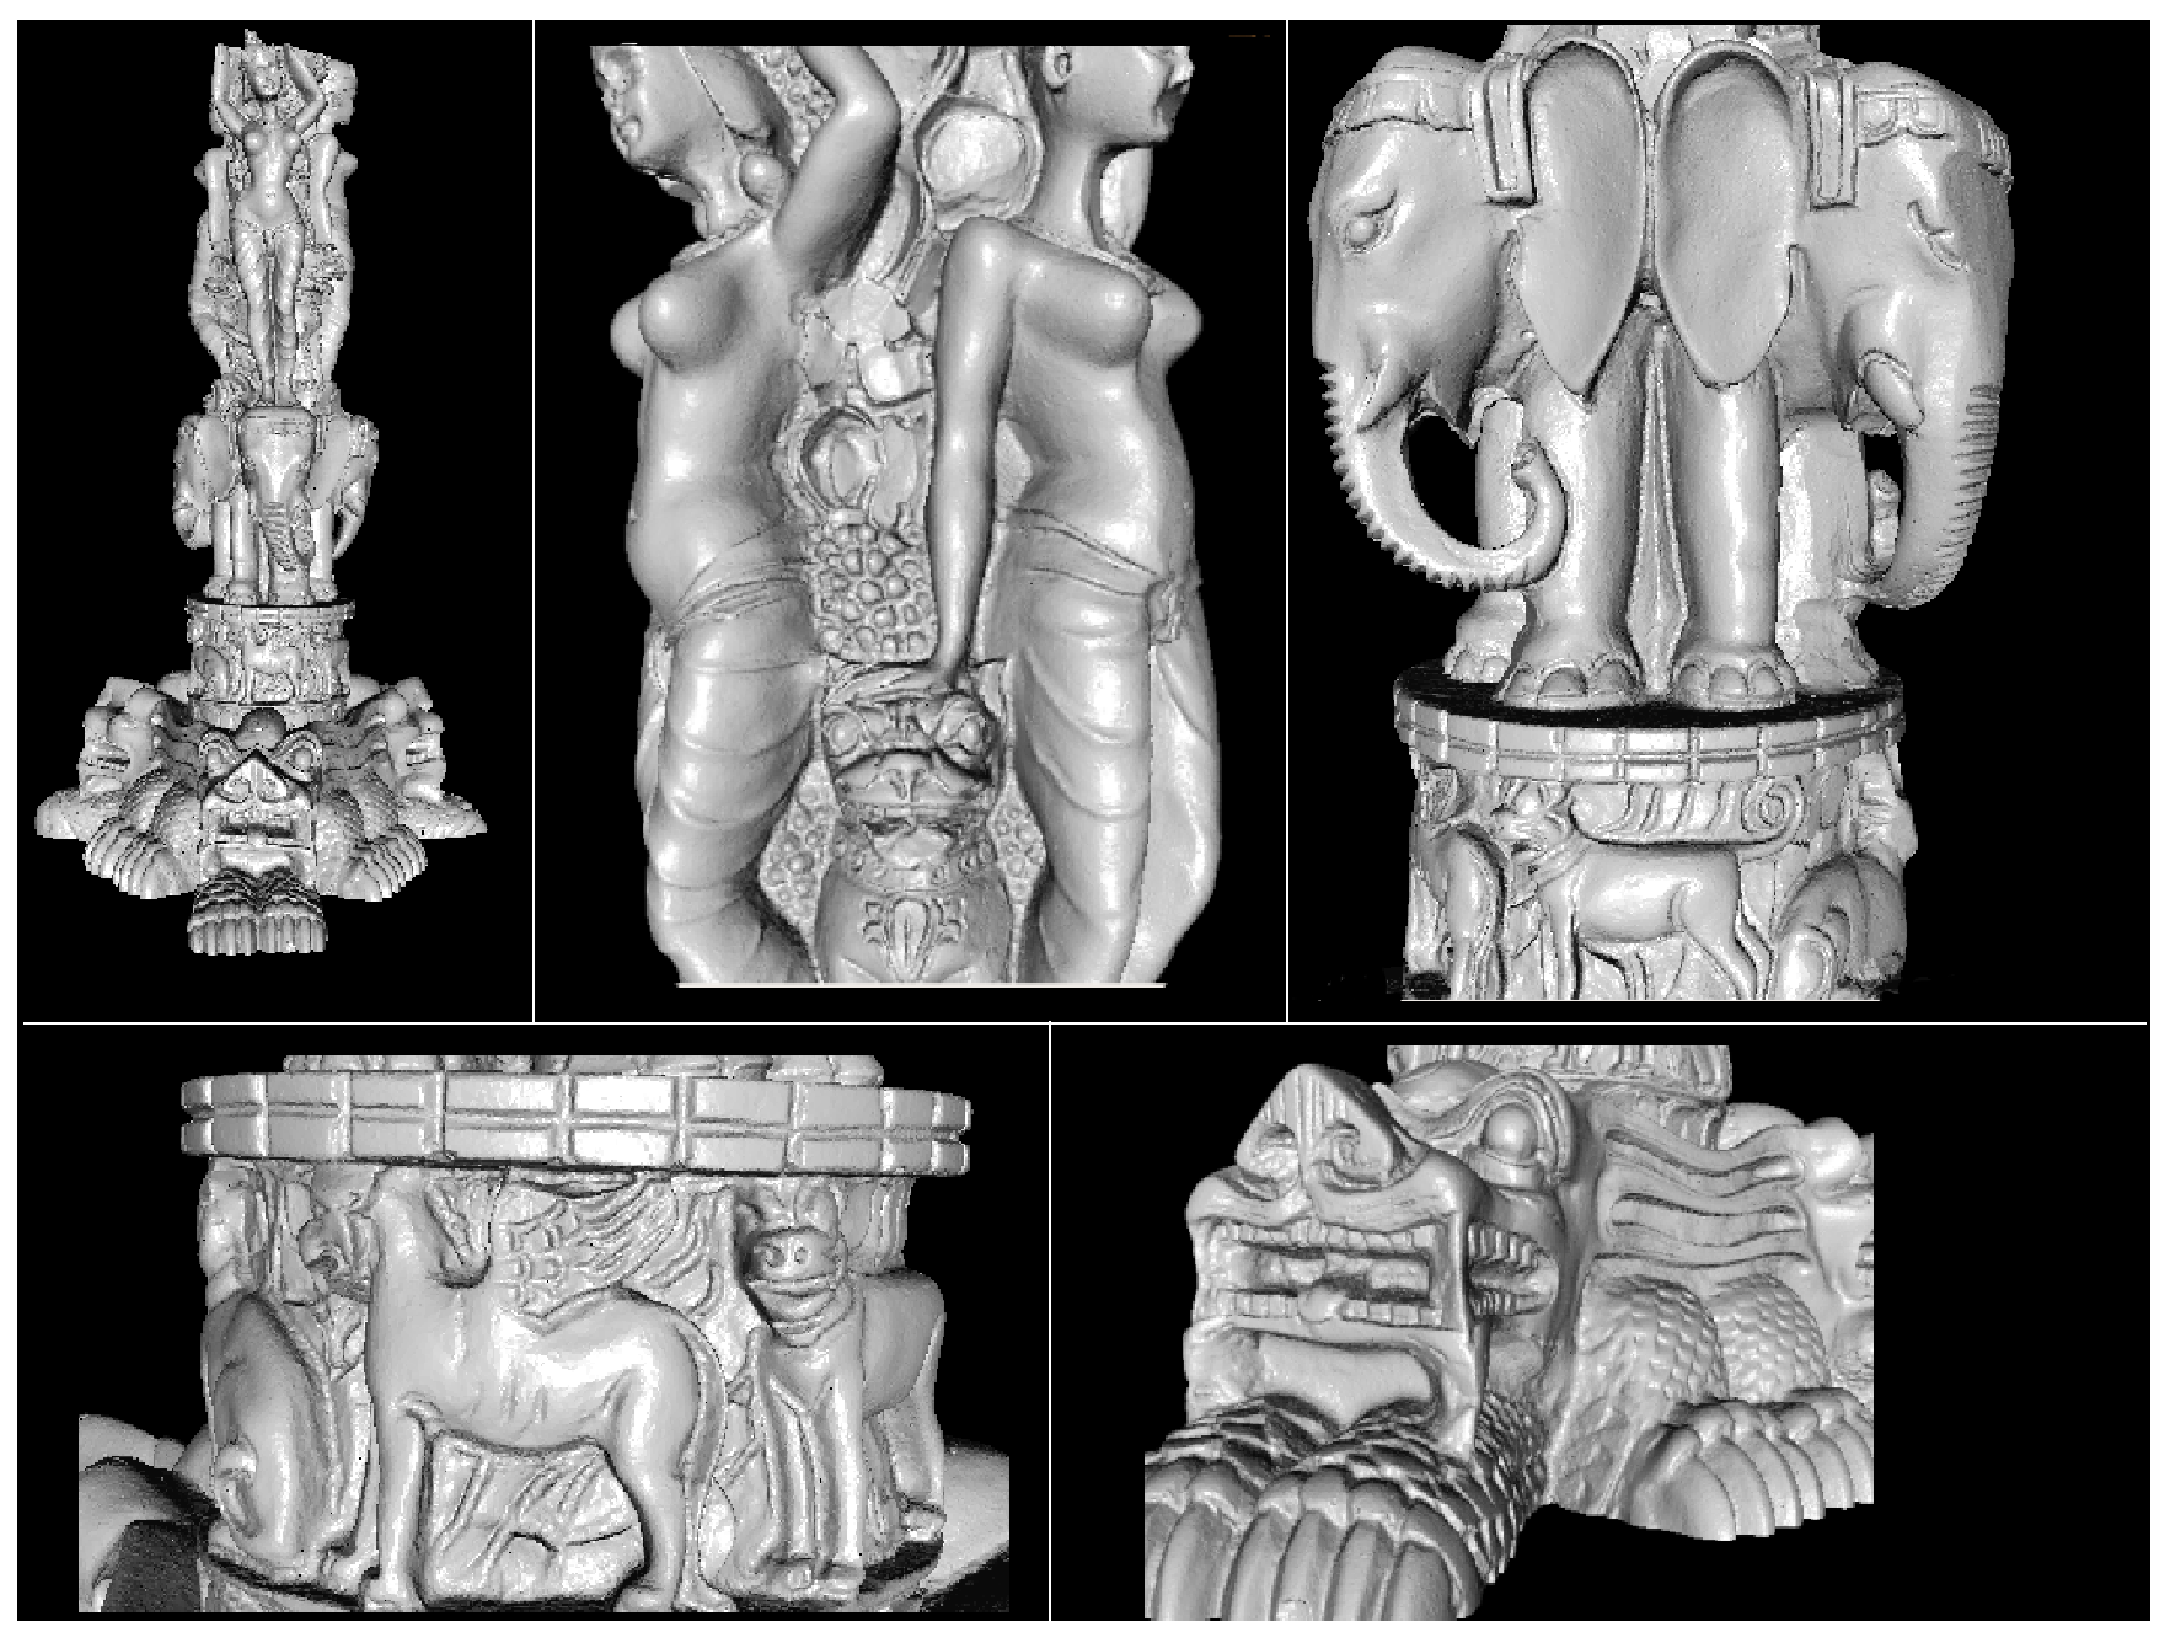
\epsfig{file=figs/thai, height = 0.6\textwidth} &
    \epsfig{file=figs/happy, height= 0.6\textwidth} \\
    Thai Statue &
    Happy Buddha \\
\end{tabular}
\epsfig{file=figs/dragon, width = 0.7\textwidth} \\
Dragon
\caption{Meshes used in experiment.   
Thai Statue (5 million vertices), Dragon (3.6 million vertices), and Happy Buddha (0.5 million vertices).}
\label{fig:3dmodels}
\end{figure}

We first introduce how we did the experiment and recorded the data. 
Then we show some interesting findings from our preliminary analysis. 
Finally, we introduce how we generate synthetic traces and 
compare them with the real traces we collected.

\section{Experiment Setup}
\label{s:user:study}
\textbf{Meshes}

Three 3D meshes are chosen from the freely available
Stanford 3D Scanning Repository:   %\footnote{http://graphics.stanford.edu/data/3Dscanrep/}:
\textit{Happy Buddha}, \textit{Dragon}, and \textit{Thai Statue}.
These meshes vary in complexity (amount of vertices), orientation, and
symmetry in space from default viewing direction. \textit{Happy Buddha} is the
simplest, is vertically oriented, and has a default viewing direction
orthogonal from the face of the Buddha. From that direction, the mesh is
asymmetric between front and back. The geometric shape of \textit{Happy Buddha} is
somewhat representative of all human-like statues. \textit{Dragon} is more complex
and is horizontally oriented. The default viewing point is from one
side of the body. Unlike \textit{Happy Buddha}, it is front-back symmetric
relative to the default viewing direction. The geometric shape of \textit{Dragon} is
somewhat representative of most mammals. \textit{Thai Statue} is the most complex
and is actually a compound mesh composed of three identical sides, each 
with three different objects: a Goddess, an elephant, and a dragon,
stacking vertically from top to bottom.  These three sides connect to
form a triangular cylinder. There are three possible default
viewing directions, one each from three corners of the triangular mesh. The
\textit{Thai Statue} is included as an example of complex compound mesh.

We replicate each mesh above twice, generating nine meshes in total.  
We added one localized visual defect, by denting a small region, to each replicated mesh 
without changing its number of vertices or faces. The reason for adding the defects will be explained later. 
The location and nature of the
defects vary between the meshes. As \textit{Happy Buddha} is
relatively simpler and has a smooth surface, its defect is
 more obvious than \textit{Dragon}
and \textit{Thai Statue}.  Defects for the later two meshes, due to the
irregular surfaces, are hard to find unless the user zooms in
considerably.

The meshes are encoded progressively and streamed over a simulated network of 320Kbps and 400ms round trip time.  

\textbf{Participants}

A total of 37 (25 male and 12 female) participants, aged 19 to 36
(mean 23), mostly from the university community participated in the
experiment. None had any visual handicaps.

\textbf{Design and Procedure}

Our experiment mimics the following general real world scenario. Customers
are shopping in an online antique store. Each product in the store has a
number of items, and each item is represented by a 3D mesh closely resembling
the corresponding real world item. These items vary in quality, and some
have visible defects. Before purchasing, customers will carefully examine the
available items for a product in order to pick the best item available for
that product category.

We designed our experiment using a simple case of the above scenario. 
Our online store has three different products,
corresponding to the three different meshes mentioned earlier. Each product
has three available items in varying quality. Two of them have visual
defects (note: defects are created without changing any mesh
characteristics). Due to the different complexity of each mesh, the defects
are easier to find in the simpler meshes (\textit{Happy Buddha}) compared to the more
complex ones (\textit{Thai Statue} and \textit{Dragon}).

\begin{figure}
    \centering
    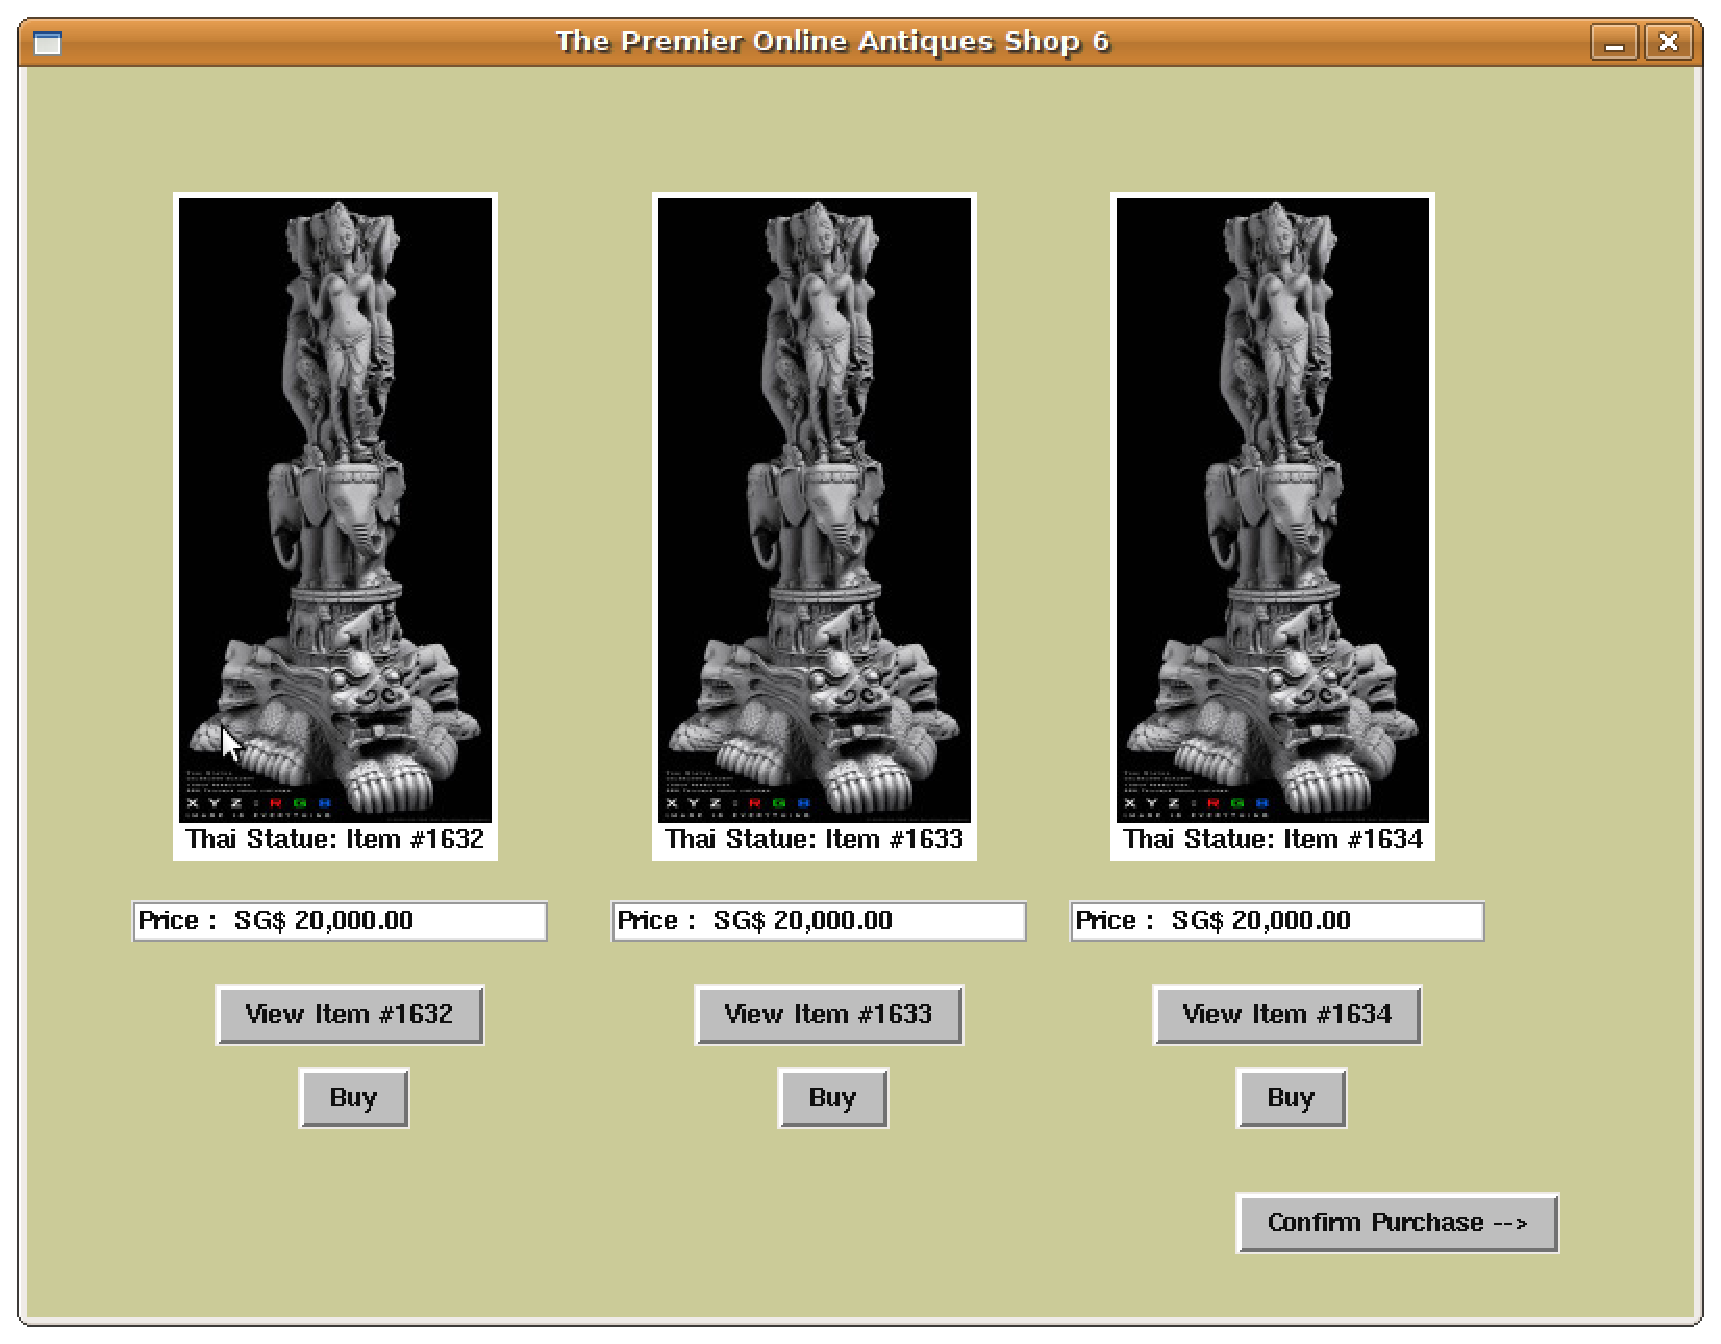
\epsfig{file=online_shop.eps, width = 0.85\textwidth}
    \caption{The user interface we used to mimic an online shop.}
    \label{f:user:shop}
\end{figure}
The participants were first instructed about the keyboard commands 
to view and interact with the 3D meshes, and given brief practice of
these commands on a simple mesh before starting the experiment. The
participants were presented with an user interface mimicking an online
catalog with three products (see Figure \ref{f:user:shop}).  For each product, images of three items 
(i.e., three versions, one original and two with defects) are shown on the screen.
The order of the products are randomized to avoid order effects.
The participants' job is to pick the best item among the three. Each item 
can be viewed in any order and if desired, multiple times.  When 
a participant selects an item, a new viewing window (width of 14cm and
height of 15cm, with a resolution of $500 \times 500$ pixels) opens, and the 3D mesh corresponding to that item is
progressively streamed and rendered in the window.  
The participants can interact freely
with the mesh until they close the window.
They would mark the item to be purchased after viewing all three items and
move on to the next product. Each participant must go through all three products to
complete the experiment.

\textbf{User Behavior Logs}

During the experiment, users' key press actions and viewpoints
were logged for off-line analysis. The representation of the viewpoints
and actions are introduced in detail as follows.

A viewpoint indicates from where and to which direction users view the mesh.
Users can change their viewpoints during the session. Changing the position of 
viewpoint is equivalent to changing the position of the mesh. 
%Therefore, from another aspect,
%users are changing the position and direction of the mesh during the session.
When the application starts, the user begins with the default viewpoint,
where the user looks at the center of the mesh (more precisely,  the center of the bounding box of the mesh)
from a distance far enough to see the whole mesh. 

We use a 6-tuple, ($x, y, z, \theta_x, \theta_y, \theta_z$) to indicate the relative position of the mesh,
%The ($x, y, z, \theta_x, \theta_y, \theta_z$) means
when the mesh is translated $x$ units right, $y$ units up, and $z$ units closer to the user (i.e. out of the screen),
and rotated $\theta_x$ degrees around $x$ axis, $\theta_y$ degrees around $y$ axis,
and $\theta_z$ degrees around $z$ axis. 
%During the rotation, the center of the mesh is not moved.
The positive directions of translation and rotation are shown in the Figure \ref{f:user:viewpoint}.
The default position is ($0, 0, 0, 0, 0, 0$).
\begin{figure}
    \centering
    \epsfig{file=viewpoint.eps, width=0.3\textwidth}
    \caption{The positive direction of translation and rotation.}
    \label{f:user:viewpoint}
\end{figure}
The position of $x$, 
$y$, and $z$ changes in unit equivalent to one tenth of the bounding length, which is the edge length
of the bounding box of the mesh. The angles of $\theta_x$, $\theta_y$, and $\theta_z$ change in unit of 10$\degree$,
and their range is $[0, 1, \cdots, 35]$.

To facilitate the analysis, we ensure the six values are all integral. 
Therefore, an action will change one of the six values by one unit.
Table \ref{t:user:action} lists out the name, the abbreviation, the result,
and the corresponding key (or key combination) of each action.\footnote{
There is a small inconsistency in our design. 
We use $\uparrow$ to move the mesh closer and $\downarrow$ to move the mesh
further. It is more like moving viewpoint than moving the mesh. 
It is the flaw in our design, but fortunately the users were used to it quickly
during the experiments.}
%When moving and zooming, 
%we move the viewpoint of the user, 
%but when rotating, we rotate the mesh. 
%In other words, when we press ALT + $rightarrow$, 
%we move ourselves to the right side of the mesh. 
%When we press $rightarrow$, however, we revolve the statue to right. 
%Fortunately, users accept this setting well and without confusion.}.

\begin{table}
    \centering
    \begin{tabular}{|c|c|c|c|c|}
        \hline
        Name & Abbreviation & Result & key/key combination \\
        \hline
        move right & MR     & $x + 1$  & ALT + $\rightarrow$\\
        move left  & ML     & $x - 1$  & ALT + $\leftarrow$\\
        move up    & MU     & $y + 1$  & ALT + $\uparrow$\\
        move down  & MD     & $y - 1$  & ALT + $\downarrow$\\
        zoom in    & ZI     & $z + 1$  & $\uparrow$\\
        zoom out   & ZO     & $z - 1$  & $\downarrow$\\
        tilt backward & TB  & $\theta_x + 10\degree$ & CTRL + $\downarrow$\\
        tilt forward & TF   & $\theta_x - 10\degree$ & CTRL + $\uparrow$\\
        revolve anticlockwise & REAN & $\theta_y + 10\degree$ & $\rightarrow$\\
        revolve clockwise & REC & $\theta_y - 10\degree$ & $\leftarrow$\\
        rotate  anticlockwise & ROAN & $\theta_z + 10\degree$ & CTRL + $\leftarrow$\\\
        rotate  clockwise & ROC &  $\theta_z - 10\degree$ & CTRL + $\rightarrow$\\
        %reset      & RS     & $all = 0$  & R \\
        quit       & Q      & quit     & Q \\
        \hline
    \end{tabular}
    \caption{Introduction of the actions.}\label{t:user:action}
\end{table}


As a result, a user session can be seen as a random process 
with viewpoints as the states. Each action transits
the system from one state to next state, until the QUIT
action terminates the session (see Figure \ref{f:user:transition} as an example). 
During the session, we record
all the user actions and the time they happened.  We call these 
records \textit{user trace}.
Moreover, ($x, y, z, \theta_x, \theta_y, \theta_z$) can be seen as a point in a 6-dimension space, and
the six axises in this space are $X$, $Y$, $Z$, $AX$, $AY$, $AZ$. 
In this sense, a session is a random walk in the 6-dimension space.
\begin{figure}
    \centering
    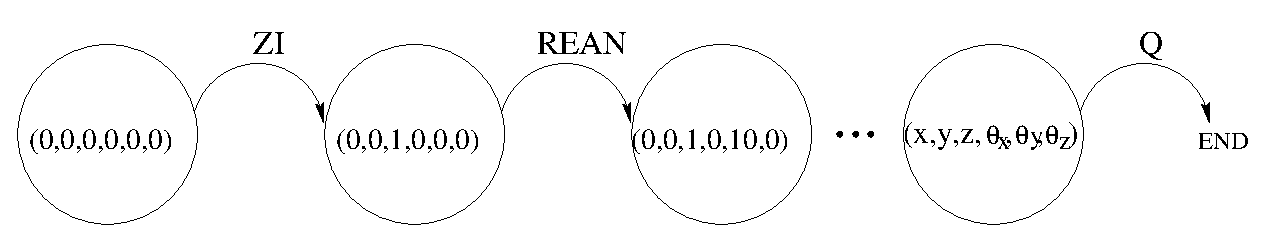
\epsfig{file=transition.eps, width=0.7\textwidth}
    \caption{An example of a user session}
    \label{f:user:transition}
\end{figure}


%\section{Results and Implications}
%In this section, we present our analysis on the user behavior. We present only on the analysis of the original (non-defect) statues, unless otherwise specified.
%In addition, we also discuss what implications these results have on system design.

\section{Preliminary Analysis}
The original purpose of our analysis on the traces we collected
is to find some patterns to help us generate the synthetic traces. 
Some preliminary findings we obtained, however, are interesting themselves and 
may lead to a potential important research topic. We found that 
in our traces we collected, the user actions are somewhat predictable.
It indicates the possibility of applying pre-fetching in our mesh streaming
system. Moreover, we found that locality exists in the traces we collected and
it means caching technique can be useful in our scenario.
In this section, we introduce these two potentially useful
by-products of our experiment in detail. 

\subsection{Predictability}
\label{ss:user:predictability}
It is interesting to see if user actions are predictable. 
If so, pre-fetching can be used to reduce response time when
users change their viewpoints. 
For example, when the connection between the 
receiver and the sender has limited bandwidth
or long delay, the requests for vertex splits of the new viewpoint 
can be sent based on the prediction before the user changes the viewpoint.
Another example is that when the client has limited
rendering power, the next viewpoint can be rendered
in advance based on the prediction to reduce the response time. 

The next action of a user, $A_n$, is a random variable with 14 possible values
(see Table \ref{t:user:action}). 
A naive way to predict the value of $A_n$ is based on the unconditional distribution 
of $A_n$, which can be estimated as the frequency of each value in the traces
we collected.  
Then, $A_n$ can be predicted as the action with highest probability.
We note this action as $a_{max}$ and its probability as $p_{max}$.
Figure \ref{f:user:frequency}
shows the frequency of occurrences of 12 different actions in the traces we collected,
displayed as a bubble chart. 
The bubble size indicates the frequency of an action occurring for a mesh.
We can see that the most frequently used actions are two revolving (rotating around y-axis). 
Table \ref{t:user:highest_probability} shows the $a_{max}$ and $p_{max}$ for all 9 meshes.
As a result, without any extra information, we can always predict that the next action is 
$a_{max}$, and the accuracy is $p_{max}$.
\begin{table}
    \centering
    \begin{tabular}{|c|c|c|}
        \hline
        Mesh              &     $a_{max}$         &    $p_{max}$ \\
        \hline
        Dragon            &     REAN              &    0.2517    \\
        Dragon1           &     REC               &    0.2237    \\
        Dragon2           &     REAN              &    0.2180    \\
        Thai              &     REAN              &    0.3292    \\
        Thai1             &     REAN              &    0.3323    \\
        Thai2             &     REC               &    0.3375    \\
        Buddha            &     REAN              &    0.3584    \\
        Buddha1           &     REAN              &    0.2707    \\
        Buddha2           &     REC               &    0.3438    \\
        \hline
    \end{tabular}
    \caption{The action with highest unconditional probability and its probability.}
    \label{t:user:highest_probability}
\end{table}
The accuracy of this prediction, however, is low. 
The best prediction we can make is for Buddha, which has the accuracy as 35.84\%. % if we guess one action and $64.34\%$ if we guess two actions
%(if the real action is one of the predictions, we consider our prediction is accurate).
The prediction could be more accurate with more information,
such as the previous action of the user and the current viewpoint of the user.
\begin{figure}[htdp!]
    \centering
    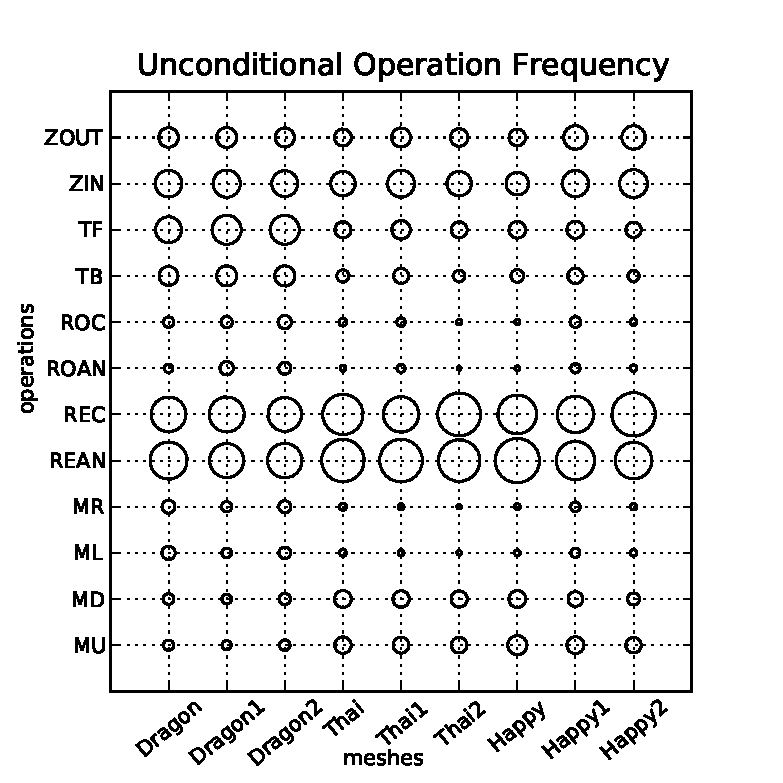
\epsfig{file=UnActionEventFrequency.eps, width=0.45\textwidth}
    \caption{The frequency of 12 actions in the traces we collected.}
    \label{f:user:frequency}
\end{figure}

\textbf{Considering Previous Action}
From the traces, we found that the value of $A_n$ highly correlates
with the value of $A_p$, the previous action taken by the user.
Figure \ref{f:user:prev_next_relation} shows the conditional 
probability of taking the next action given the previous action
%for \textit{Thai Statue}.
for the three meshes.
The shaded diagonal shows that the same action has the 
significantly larger probability (e.g., more than 0.93 for revolving) 
of being taken next. %The other meshes exhibit the similar pattern. 
\begin{figure}[htp!]
    \centering
    \begin{tabular}{c}
        \epsfig{file=figs/traceHistogram0/Inter-operationprobability-hugenormal.eps, width=0.45\textwidth}\\
        \epsfig{file=figs/traceHistogram0/Inter-operationprobability-dragonnormal.eps, width=0.45\textwidth}\\
        \epsfig{file=figs/traceHistogram0/Inter-operationprobability-happynormal.eps, width=0.45\textwidth}
    \end{tabular}
\caption{The conditional probability of next action if the previous action is given.}
\label{f:user:prev_next_relation}
\end{figure}

According to this observation, 
we categorized the actions into two types: \textit{repeat}, \textit{non-repeat} and use 
$P_{repeat}$ to represent the probability to repeat the previous action.
Then we can predict the next action by choosing ``repeat'' unconditionally.
The $P_{repeat}$ for three meshes can be seen in Figure \ref{f:user:cont_prob}.
We can see that always choosing ``repeat'' as the prediction has high accuracy 
(larger than $80\%$ for all meshes). 
\begin{figure}[htdp!]
    \centering
    \epsfig{file=cont_prob_9.eps, width=0.6\textwidth}
    \caption{The probability of repeating the previous action for 9 meshes.}
    \label{f:user:cont_prob}
\end{figure}

\begin{figure}
    \centering
    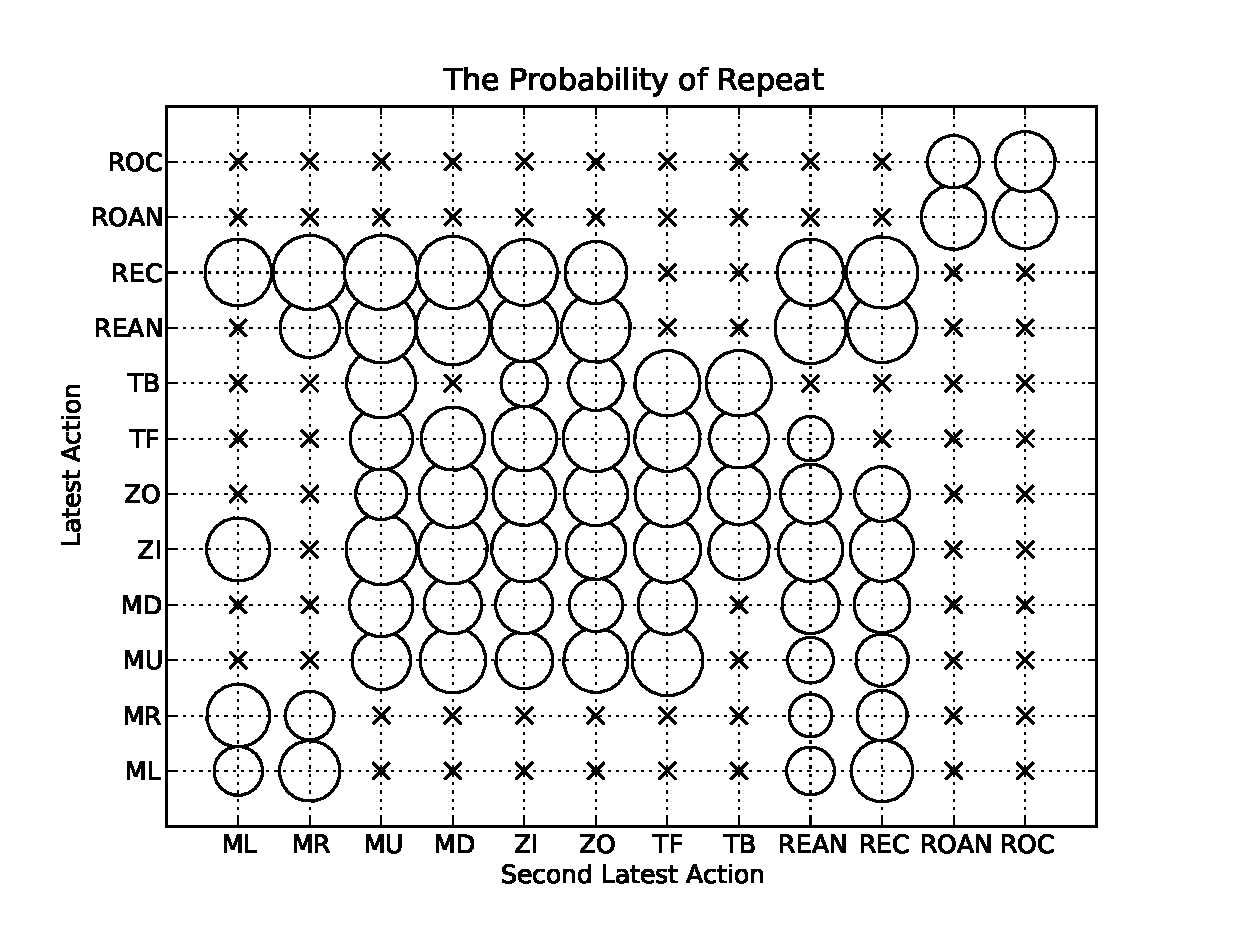
\epsfig{file=happy_2.eps, width=0.55\textwidth}\\
    Buddha\\
    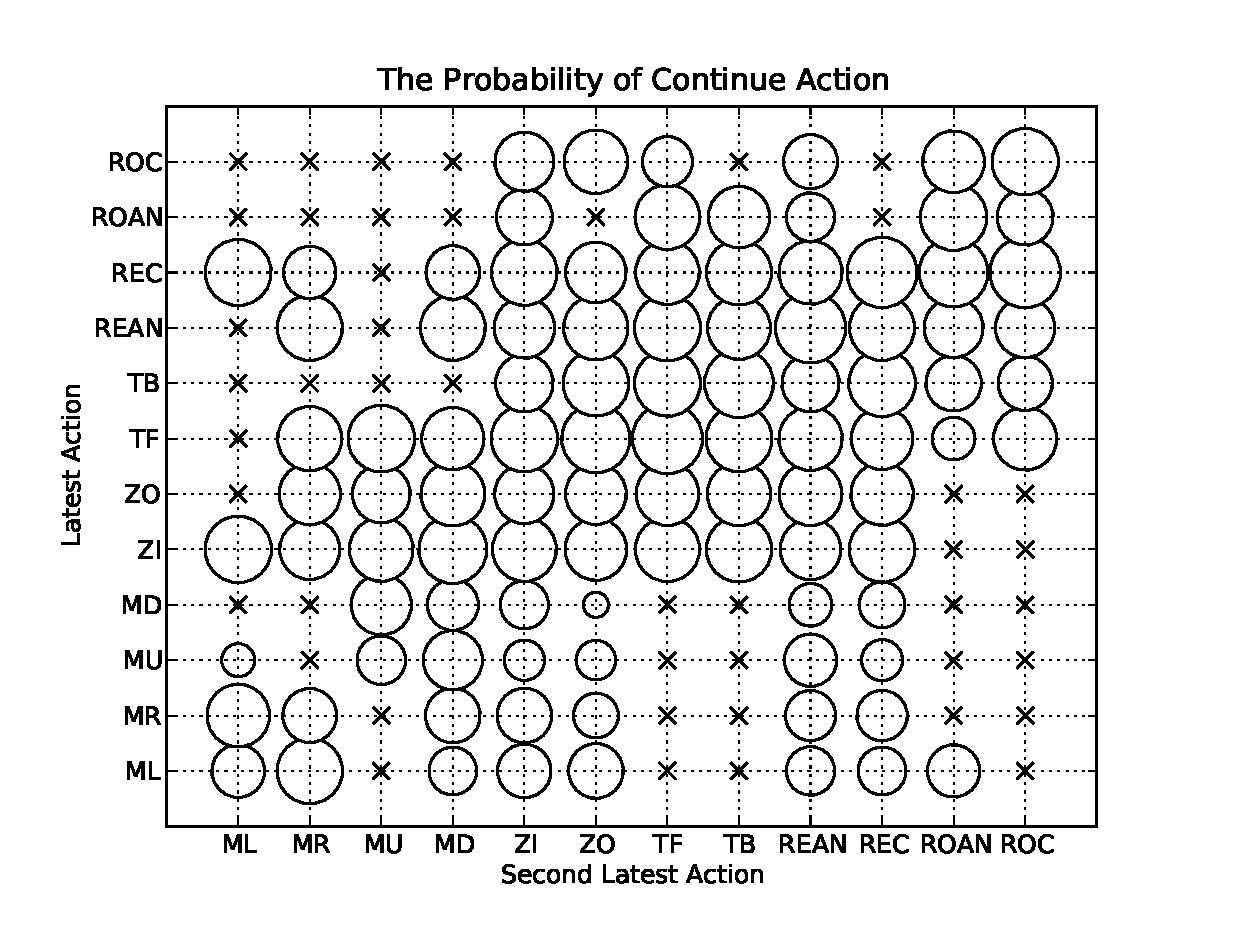
\epsfig{file=dragon_2.eps, width=0.55\textwidth}\\
    Dragon\\
    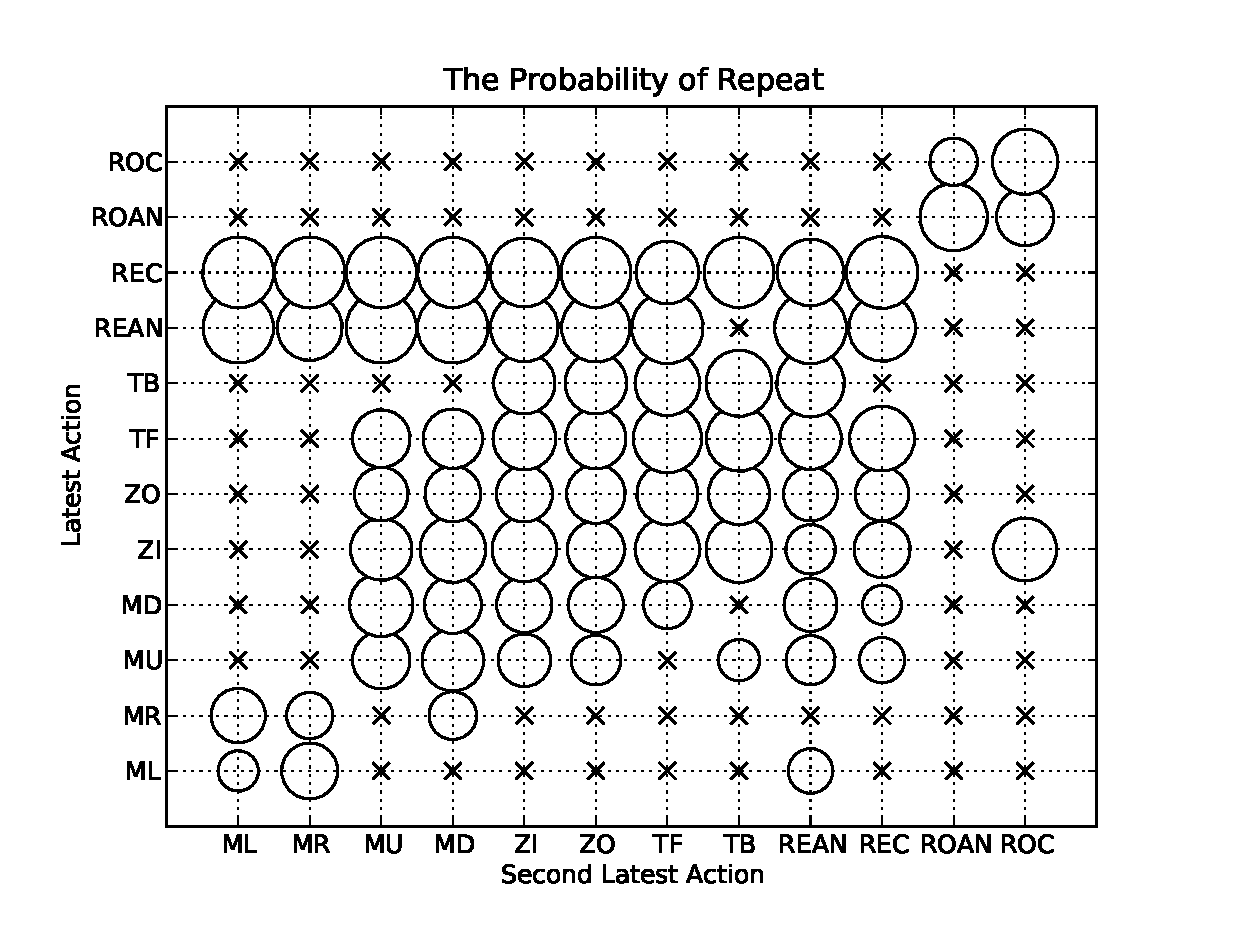
\epsfig{file=thai_2.eps, width=0.55\textwidth}\\
    Thai Statue
    \caption[The probability of repeating the previous action for each combination of previous two actions (Thai Mesh).]
    {The probability of repeating the previous action for each combination of previous two actions (Thai Mesh).
    'x' means that the sample size of this combination is too small (less than 10 samples) to obtain reliable probability.}
    \label{f:user:prev2}
\end{figure}
Next, we check whether it helps to consider one more action, the second previous action. 
The $P_{repeat}$ under different combination of
previous two actions for Thai Mesh is shown in Figure \ref{f:user:prev2}.
In this figure, we can see that the second previous action does affect the 
$P_{repeat}$, but the effect is much less significant than the previous action. 
Moreover, we found that in around 99.9\% of the combinations, 
repeating the previous action still has the largest probability,
so the prediction based on previous action and the one based on previous two actions are the same in
most of the cases. 
Therefore, we conclude that considering only the previous action is enough for the prediction.

\textbf{Considering Viewpoint} 
The other method to improve the prediction accuracy is to consider the current viewpoint of the user.
We compute the conditional distribution of next action $A_n$ on each viewpoint, 
and always choose the action with the highest conditional probability as the prediction.

Since we estimate the probability of an action as the frequency 
of its occurrence in the real traces, 
enough number of samples are required to give reliable results. 
By analyzing the traces we collected, we found that majority of the samples are 
on a small proportion of viewpoints, and for the rest viewpoints, we have few
samples (See Figure \ref{f:user:sample_size_1}).
\begin{figure}
    \centering
    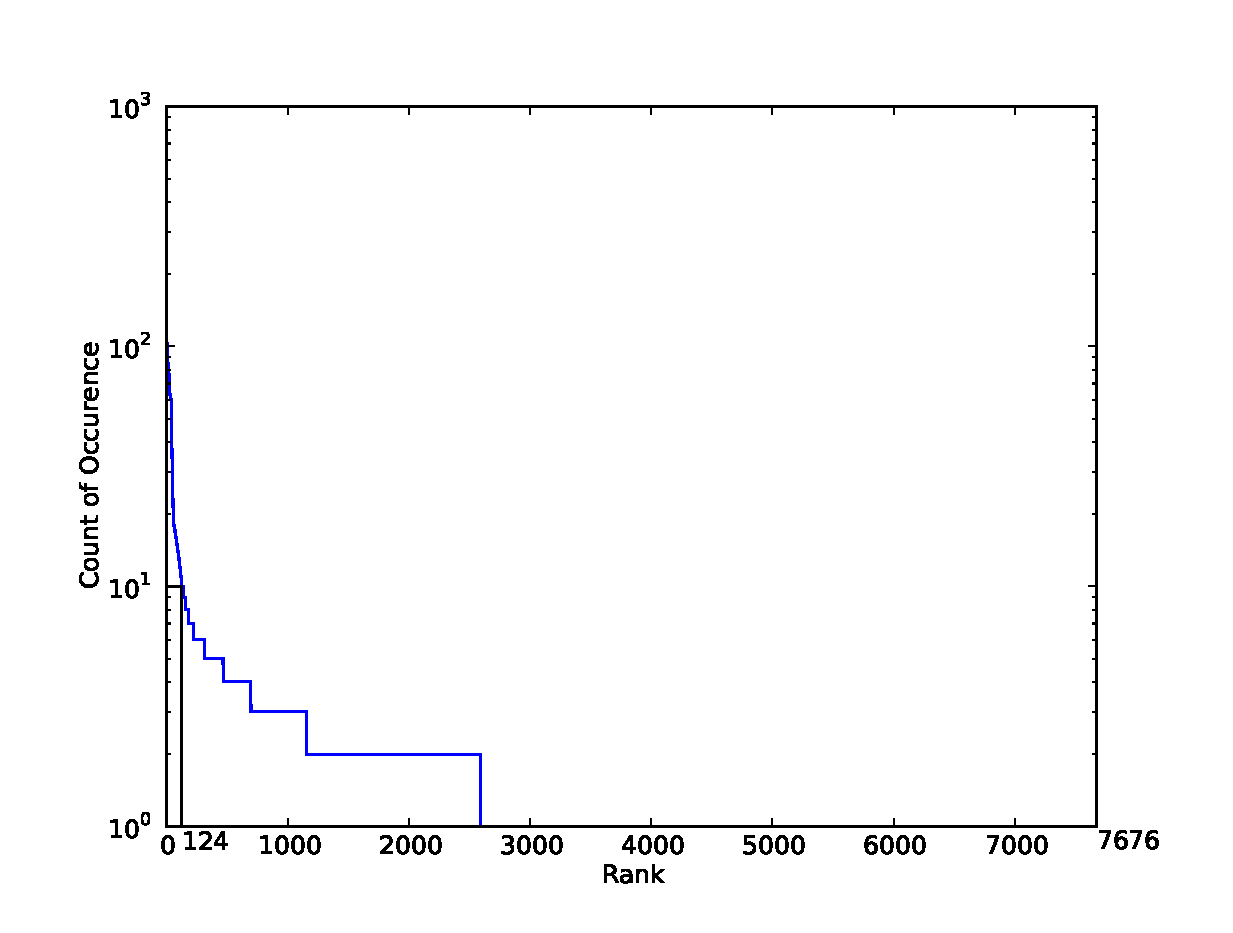
\epsfig{file=happy_sample_size_1.eps, width=0.55\textwidth}\\
    Buddha\\
    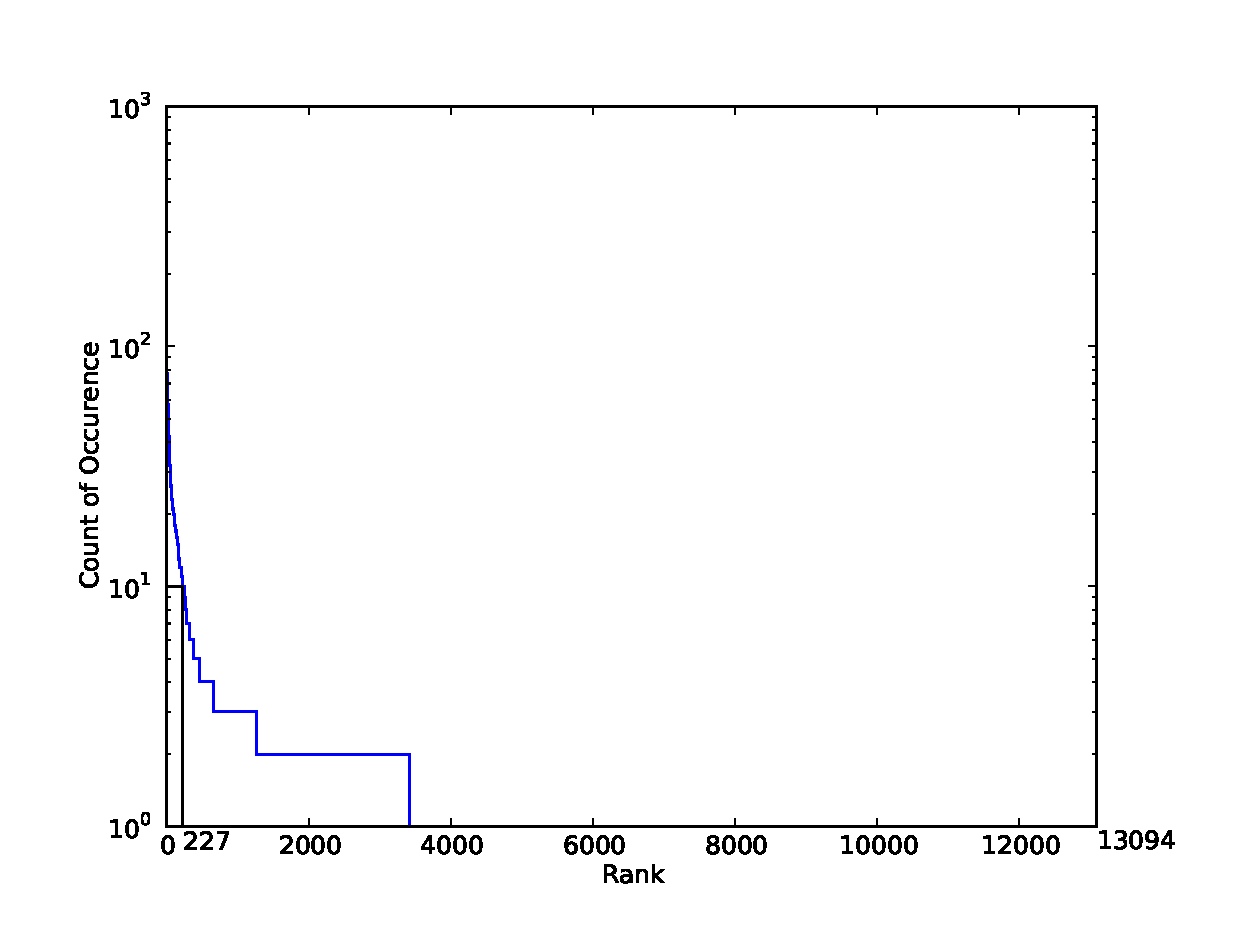
\epsfig{file=dragon_sample_size_1.eps, width=0.55\textwidth}\\
    Dragon\\
    \epsfig{file=thai_sample_size_1.eps, width=0.55\textwidth}\\
    Thai Statue
    \caption{The number of samples on all viewpoints, and the viewpoints are sorted from the most popular to the least popular.}
    \label{f:user:sample_size_1}
\end{figure}
Including the viewpoints having few samples may exaggerate the accuracy.
For example, the predictions on the viewpoints having one sample are 
always true, which is not realistic.
Therefore, we ignore all those viewpoints with less than 10 samples.
Figure \ref{f:user:accuracy_comp} (labelled ``Vp'') shows the accuracy of this method.
We can see that this method has lower accuracy than the one based on previous action.

\textbf{Considering Viewpoint and Previous Action}
To improve the accuracy, we could consider both viewpoint and previous action.
%Now we consider both current viewpoint and  previous action.
Similarly, we compute the conditional distribution of next action $A_n$ for each combination. 
Then we always choose the action with highest conditional probability as the prediction.

The same problem of lacking samples exists for most combinations (See Figure \ref{f:user:sample_size_2}).
\begin{figure}
    \centering
    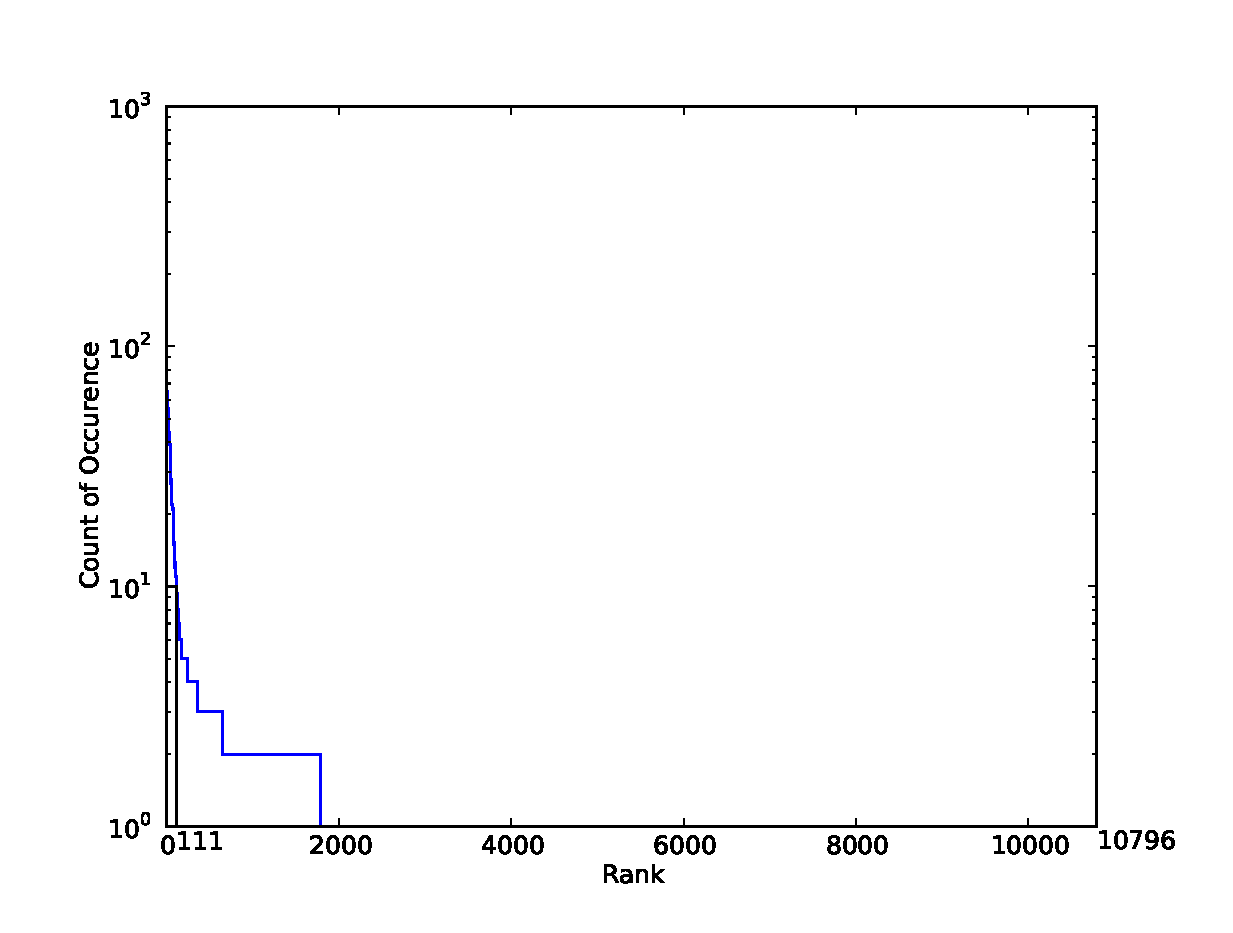
\epsfig{file=happy_sample_size_2.eps, width=0.55\textwidth}\\
    Buddha\\
    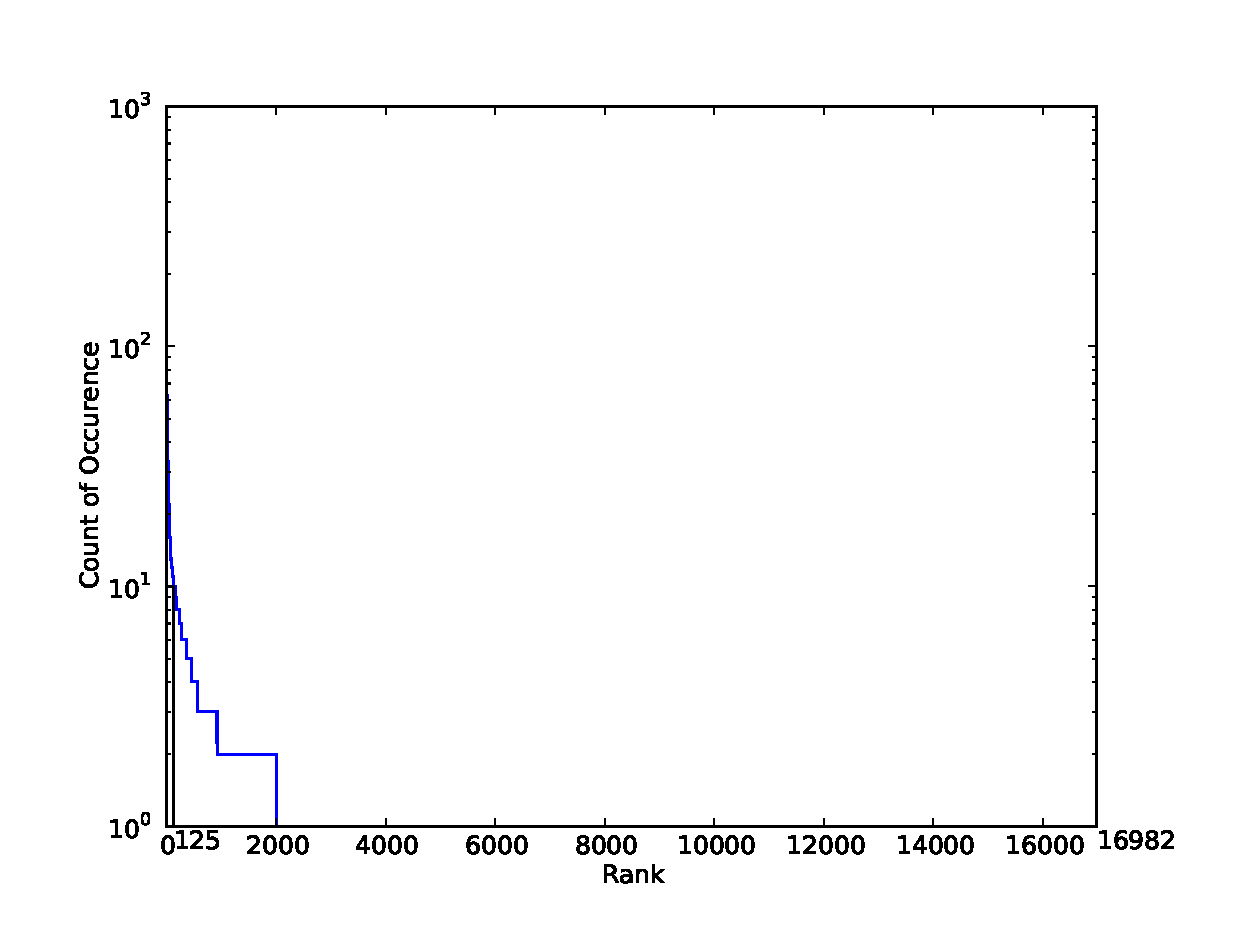
\epsfig{file=dragon_sample_size_2.eps, width=0.55\textwidth}\\
    Dragon\\
    \epsfig{file=thai_sample_size_2.eps, width=0.55\textwidth}\\
    Thai Statue
    \caption{The number of samples on all combinations of viewpoint and previous action, and the combinations are sorted from the most popular to the least popular.}
    \label{f:user:sample_size_2}
\end{figure}
We ignore those combinations with  less than 10 samples.
The accuracy of this method can be seen in Figure \ref{f:user:accuracy_comp}.
This method has the highest accuracy among the four methods.

We compare the four methods in Figure \ref{f:user:accuracy_comp} for three meshes\footnote{
To increase the sample size, we aggregate the data of the three version of the same mesh together.
It is reasonable because the meshes having a defect are almost identical to the original one, 
and users do not know which one has defect in advance. Therefore, their behavior on 
all three versions of the same mesh are similar.}.
We have found that in our scenario the user actions are somewhat predictable and the prediction is simple.
Predicting the next action be the same as the previous one without considering
any extra information can achieve good enough accuracy in our cases. 
Considering both previous action and viewpoint has the highest accuracy,
but it depends on the statistics of user behavior and differs on every mesh. 
Hence, it can only be done when enough user traces are already collected for a specific mesh. 
The slightly better accuracy may not justify the much higher complexity.
The interesting finding provides a preliminary evidence that pre-fetching can be useful
in mesh streaming.
%This is an interesting finding, but due to the small number of traces and the specific scenario we chose,
%we cannot achieve general conclusion yet. Further study with more experiments and more participants could 
%be an interesting future work.
\begin{figure}
    \centering
    \epsfig{file=accuracy_comp.eps, width=0.65\textwidth}
    \caption{The accuracy of four prediction methods.}
    \label{f:user:accuracy_comp}
\end{figure}

\subsection{Guiding Caching with User Traces}
%According to our observations, parts of a mesh have different popularity. 
%popular parts of the mesh. 
Caching techniques are used to spend limited resources (such as 
servers, memories, and network bandwidth) on the most popular requested 
data to improve the system performance. 
Hence, how effective a caching system can be depends on the access pattern
of users. For example, if most user requests concentrate on a small 
part of the data, then a small cache can significantly improve the 
system performance. On the contrary, if all data are equally important,
then caching is much less effective. Therefore, to study user traces
is crucial in designing a caching system.
In this section, based on the analysis of the traces we collected, 
we show that in our case how caching is useful in three different scenarios:
(i) progressive mesh streaming, (ii) remote rendering, and (iii) 
mesh rendering.
%In this section, we show that the user traces exhibit access
%patterns that can lead to efficient caching in three different scenarios.

\textbf{Caching for Mesh Streaming}.
%In progressive mesh streaming, vertex splits are often grouped into chunks
%for transmission. These chunks can be cached at a proxy to reduce server overhead.
%To study the usefulness of proxy caching, we look at the access pattern to chunks. 
In progressive mesh streaming, vertex splits can be cached at a proxy to reduce server overhead.
Usually, caching proxy has limited memory (or it can only provide limited memory for a certain mesh),
so only a small part of the vertex splits can be stored. To study the usefulness of proxy caching,
we look at the access pattern to vertex splits.

We first replay the log of actions from the users, and generate
a list of vertex splits accessed  by users during the experiment.  
From these vertex split requesting traces, we count
the number of times each vertex split is accessed.  We then sort the vertex splits
in decreasing order of the access count, and plot the cumulative
access count versus rank in Figure \ref{fig:CDF}(a).  We normalize both axes to between 0 and 1
so that we can plot all three meshes on the same graph.  
Figure \ref{fig:CDF}(a) shows how many requests (in percentage) we can satisfy (i.e., hit rate) 
by storing the most frequently requested chunks in a proxy. 
The x-axis denotes the number of vertex splits stored in the proxy, 
as a fraction of total number of vertex splits requested
(note: not the total number of all vertex splits).
It can be observed that by building a static
cache that stores 20\% of the most frequently accessed
vertex splits, the proxy can achieve more than 70\% hit rate for
\textit{Thai Statue} and \textit{Dragon}, and 55\% for 
\textit{Happy Buddha}.

    \begin{figure}[htp]
        \begin{center}
        \begin{tabular}{cc}
            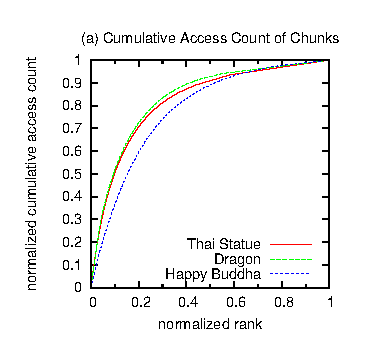
\epsfig{file=RequestCountCDF2.eps, width = 0.45\textwidth}&
            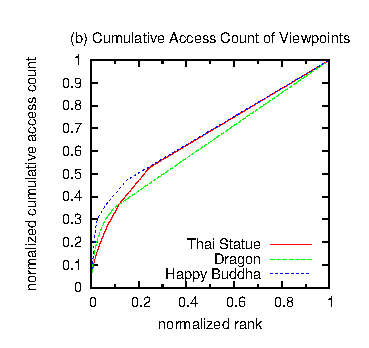
\epsfig{file=vpCDFpercentage.eps, width = 0.45\textwidth}\\
        \end{tabular}
    \end{center}
        %\caption{Normalized cumulative access count of mesh (left: chunks, right: pre-rendered images) versus rank.\label{fig:CDF}}
        \caption{Cumulative Access Count versus Rank\label{fig:CDF}}
    \end{figure}

\textbf{Caching of Remote Rendering.}
For rendering on mobile devices \cite{bao06remote} or for 
protection of mesh data \cite{koller04scanview}, 
the server could send a rendered image directly according to the users' viewpoint.
In this
scenario, the caching proxy can cache the rendered images.  We can
similarly find the viewpoints ``visited'' by the most users.  A
viewpoint visited multiple times by the same user is only counted
once, since the user can keep the received image locally and need not
request it the second time.  Figure \ref{fig:CDF}(b) shows a plot
similar to Figure \ref{fig:CDF}(a), but for access frequency of 
viewpoints.  The figure shows the hit rate at the caching proxy 
if we choose to store pre-rendered images corresponding to the
most frequently accessed viewpoints.
The distribution is not as skewed as access count for chunks, 
but still, caching the rendered images for 20\% of the most 
frequently accessed viewpoints can yield 40 - 50\% hit rate
in our scenario.

\textbf{Caching of Vertices and Pixels.}
Caching mesh data in graphic card memory 
(e.g. using VBO (Vertex Buffer Object) and PBO (Pixel Buffer Object) supported in OpenGL), 
could significantly increase the rendering speed when the memory bandwidth is the bottleneck.
For graphic cards without enough memory to store the whole mesh, we could just store the most frequently viewed part of the mesh
in the graphic card memory. 
%Since changing the stored data in graphic card memory is usually expensive, so 
%the stored data cannot be adaptively changed.

We replay all the user traces, and whenever the viewpoint changes 
%count the number of times each face is viewed.
we add the access number of the visible faces by one. 
Therefore, the access number of a face is the count of viewpoints at 
which it is visible (revisiting to a previously visited viewpoint is also counted
since the mesh will still be rendered). 
We normalized the number of views of each face and visualize them with
 a heat map (Figure \ref{fig:heat_map}). 
%duration of different parts of the ``Happy Buddha'' mesh obtained by
%replaying all the traces we collected.  
We can see that the most frequently viewed region of \textit{Happy Buddha} (viewed 4205 times) is 
the base between the two legs because it is visible from both the front and the back.
%Next, we sort the faces in decreasing order of the access count, and draw 
Figure \ref{fig:face_hit_rate} plots the normalized cumulative view count of faces versus rank, 
similar to Figure \ref{fig:CDF}. We can see that the locality is slightly less than
that in the previous two scenarios, but for \textit{Happy Buddha} and \textit{Thai Statue}, hit rate of 40\%  can be achieved
%accesses can be satisfied 
by storing 20\% of the most frequently viewed faces in the graphic card memory.
The mesh \textit{Dragon} has the least locality. We hypothesize that this is because %related to two reasons:
people tend to view \textit{Dragon} at many different viewpoints due to its complex shape,
%Hence, it is relatively less common for users to come back to viewpoints previously visited. 
leading to more evenly distributed viewpoints around the mesh.
%and faces have even chances to be viewed.
%    \begin{figure}[htbp]
%        \centering
%        \begin{tabular}{cc}
%        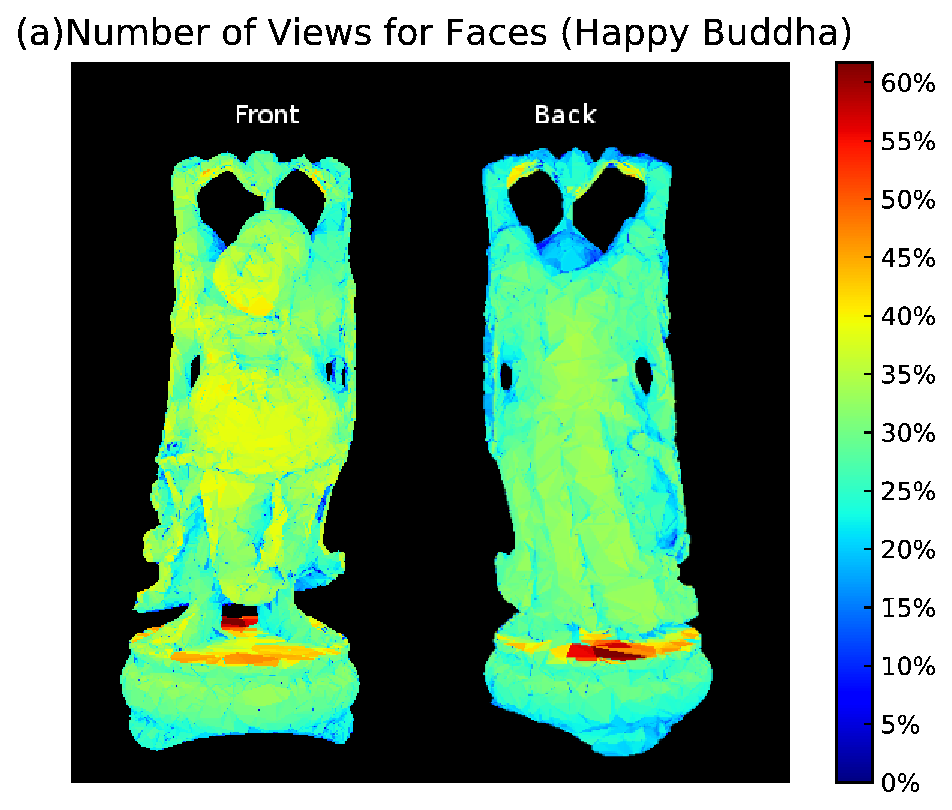
\epsfig{file=heatmap2.eps, width =0.5\textwidth}&
%        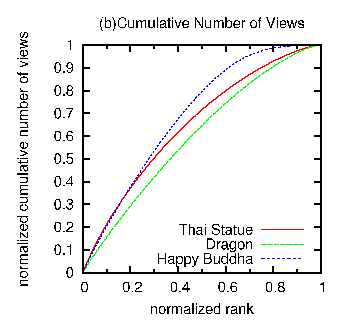
\epsfig{file=faceCache.eps, width = 0.5\textwidth}\\
%    \end{tabular}
%        \caption{(a)The normalized number of views for each face. (b) The hit rate when we save part of the faces in the graphic card.\label{fig:heat_map}}
%    \end{figure}
\begin{figure}[htp!]
    \centering
\begin{tabular}{c}
 \epsfig{file=heatmap_buddha_bw.eps, height=0.45\textwidth} \\
 \epsfig{file=heatmap_dragon_bw.eps, height=0.45\textwidth} \\
 \epsfig{file=heatmap_thai_bw.eps,   height=0.45\textwidth} 
\end{tabular}
\caption{The normalized number of views for each face. \label{fig:heat_map}}
\end{figure}

\begin{figure}[htdp!]
    \centering
 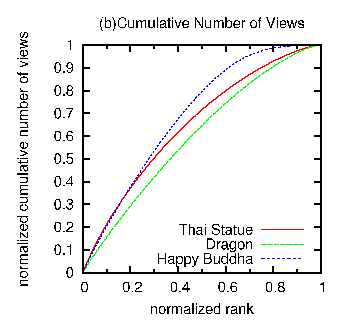
\epsfig{file=faceCache.eps, height=0.45\textwidth}
\caption{The hit rate when we save part of the faces in the graphic card.\label{fig:face_hit_rate}}
\end{figure}

%These finding are still preliminary due to the limited number of traces we obtained. More user traces
%could be obtained in the future to obtain more mature results.

\section{Generating Synthetic Traces}
\label{s:user:synthetic}
To evaluate the effectiveness and performance of a system, we often need many user traces. 
It is expensive to collect a large number of real traces. 
A cheaper way is to consider a user trace as a Markov chain
and derive the transition matrix from the collected traces.
Then following the transition matrix, we can generate as many traces as we want.

As we introduced in Section \ref{s:user:study}, a user session is a random process 
with viewpoints as the states. Each action transits
the system from one state to next state, until the session is terminated
(see Figure \ref{f:user:transition} as an example). 
To generate a synthetic trace, we first need to determine the session length, i.e. how long
the user spent in viewing on this mesh. Then we begin from the default viewpoint and keep
determining the next action until the session time is expired. For each action, we need 
to determine two things: when and what is the next action. In this section we first introduce
how we determine the session length and the interval between two actions, named \emph{think time},
and then we introduce how we choose the next action based on current state in detail.

\subsection{Session Length}
\label{ss:user:session}
Session length refers to the time each user spends in viewing a mesh. 
Generally, the session length is short, with the average values of 107s, 76s, 47s for \textit{Thai Statue}, 
\textit{Dragon}, and \textit{Happy Buddha}, respectively (see Table \ref{t:TimeTable}). 
Figure \ref{fig:session-length}(a) shows the distribution. 
The session length decreases with complexity of the meshes, as expected. 
The session length fits the \textit{log-normal} distribution.
For example, the session length of Thai Statue follows a log-normal
distribution with $\mu=18.23$, $\sigma = 0.754$ and the unit is ${\mu}s$.
When we generate a synthetic trace, we determine the session length by generating a random number following 
the log-normal distribution with parameter derived from the real traces.

\begin{figure}[htp]
\begin{center}
\begin{tabular}{c}
\epsfig{file=figs/unconditionalThinkTimeResults/sessionLengthdistribution.eps, width=0.55\textwidth,angle=270}
\end{tabular}
\caption{\label{fig:session-length} Distribution of Session Length}
\end{center}
\end{figure}

\begin{table}[hbp!]
\begin{center}
\begin{tabular}{|c|c|c|c|c|c|}
\hline 
Mesh&\multicolumn{2}{c|}{Session Length}&\multicolumn{2}{c|}{Think Time}\\
\cline{2-5}
&Mean($s$)&Max($s$)&Mean($ms$)&Max($s$)\\
\hline
Thai Statue&107&376&593&25\\
\hline
Dragon&76&272&574&20\\
\hline
Happy Buddha&47&98&403&13\\
\hline
\end{tabular}
\caption{Session Length and Think Time\label{t:TimeTable}}
\end{center}
\end{table}

%\begin{table}[hbp!]
%	\centering
%	  \caption{Session Length Stastistics}
%		\begin{tabular}{|c|c|c|c|}
%		\hline
%		Model&Sample Size&Mean(s)&Max(s)\\
%		\hline
%		Thai Statue&60&107&376\\
%		\hline
%		Dragon&63&76&272\\
%		\hline
%		Happy Buddha&39&47&98\\
%		\hline
%		\end{tabular}
%		\label{SessionTable}
%\end{table}

\subsection{Think Time}
\label{ss:user:thinktime}
We refer to the time between two actions as \textit{think time}. 
We find that think time follows similar distributions for all of the three meshes (Figure \ref{fig:think-time}(a)). 
%There is a jump in the curve of think time distribution for all the three meshes -- 
%about 5\% of the think time clusters around 0.5 seconds. 
%We hypothesize that this is related to the 0.4-second round trip time in our experiments. 
%After a user performs an action, it takes 0.4 seconds before the user can see progressive refinement of the mesh
%(although the system responses to the change in viewpoint \textit{immediately}). 
%Some users might wait for the refinement to come before the next action.
The mean and maximum think time are shown in Table \ref{t:TimeTable}. 
We note that the maximum is up to 50 times larger than the mean, but about 90\% of the think time is smaller than a second. 
\begin{figure}[htp]
\begin{center}
\begin{tabular}{cc}
\epsfig{file=figs/unconditionalThinkTimeResults/ThinkTimeDistribution3.eps, width=0.45\textwidth, angle = 270}&
\epsfig{file=figs/conditionalThinkTimeResults1/ConditionalThinkTimeDistribution1hugenormal.eps, width=0.45\textwidth, angle = 270}\\
\end{tabular}
\caption{\label{fig:think-time} Think Time (x-axis in log scale).}
\end{center}
\end{figure}

A simple method to determine the think time is following the distribution
we derived from the traces, without considering the current state.
This may be not accurate since the current viewpoint may affect the 
distribution of the think time. Furthermore, people tends to repeat the same
action quickly, and usually takes longer time if they change to another action.
Therefore, whether next action is repeating last action is also an factor to be considered.

To investigate the relation between think time and viewpoints, we
classify the viewpoints into 4 regions: front-far (FF), front-near
(FN), back-far (BF), and back-near (BN), based on \textit{front/back} and
\textit{far/near}. We find that the effect of region on think time distribution is not
apparent \ref{fig:think-time}(b)).  Hence, for simplicity we ignore the effect
of viewpoint during determining think time.

Next, we examine the effect of repeating or non-repeating the previous action. 
%it is reasonable to assume think time is small when user just repeat 
%the previous action and the think time tends to be big when user change to another action.
Figure \ref{f:user:thinktime} shows %this assumption is correct.
think time tends to be much shorter when users repeat the previous action.
Hence, during the synthetic trace generating, we use the respective distribution after
we decide the next action. Next, we introduce how we determine the next action.
\begin{figure}
    \centering
    \epsfig{file=thinktime.eps, width=0.5\textwidth}
    \caption{Think time is smaller when user repeat the previous action.}
    \label{f:user:thinktime}
\end{figure}

\subsection{Next Action}
We decide the next action based the Markov chain method.
The viewpoint, represented as a 6-tuple: ($x, y, z, \theta_x, \theta_y, \theta_z$)
as introduced in Section \ref{s:user:study}, can be defined as the states in the Markov chain.
According to the observation that the previous actions highly affects the next action
(Section \ref{ss:user:predictability}), it is not a first order Markov chain because
the previous states affect the transition probability. 
It, however, is not practical to consider the whole history before. 
To make the analysis possible, we consider only one step before and assume
``(previous state, current state)'' decides ``next state''. In other words, 
it is a second order Markov chain. 
As we introduced in Section \ref{ss:user:predictability}, the latest action affects the most, so
this simplification is reasonable.

We can reduce the second order Markov chain to first order by defining the current state as
(previous viewpoint, current viewpoint). After a user action, the new state becomes 
(current viewpoint, next viewpoint) (See Figure \ref{f:user:reduction}(a)). 
Then, the transition probability only depends on the current state.
Notice that (previous viewpoint, current viewpoint) is equivalent to (current viewpoint, previous action), 
so we finally define the state to be ($x, y, z, \theta_x, \theta_y, \theta_z, A_p$). 
(See Figure \ref{f:user:reduction}(b)).
\begin{figure}
    \centering
    \epsfig{file=reduction.eps, width=0.6\textwidth}
    \caption[Two equivalent definitions of state.]{(a), State = (previous viewpoint, current viewpoint); (b), State = ($x, y, z, \theta_x, \theta_y, \theta_z, A_p$)}
    \label{f:user:reduction}
\end{figure}

Each record in the user traces can be seen as a sample of this random process.
From these samples, we can compute the transition probability between two states, and hence
the transition matrix, with which we can generate synthetic traces.

This method, however, has limitations when the number of collected traces is small. First, if a viewpoint is 
never accessed by the real traces, it will not accessed by synthetic traces either. Therefore, no matter how
many synthetic traces are generated, the number of accessed viewpoints is upper-bounded. 
Second, due to the large sample space and limited number of samples, most of the states has only one sample
(See Figure \ref{f:user:sample_size_2}). 
In other words, in the transition matrix, the next action for most states are determined. 
As a result, after several steps, the synthetic trace follows the exact path as one of the real traces. Therefore, the synthetic traces are not random enough.

To address these two limitations, we propose a method to generate traces that are more random in the next section.
It is based on a simplified model, which does not directly derive and follow the transition matrix.

\subsection{Simplified Model}
To generate a synthetic trace, we need to determine the probability of each possible $A_n$ based on current
state ($x,y,z,\theta_x,\theta_y,\theta_z,A_p$). Due to the limited number of samples, we cannot obtain the reliable
transition probability for most of the states. As a result, we need to find a new way to determine the 
conditional distribution of $A_n$.

To address the problem of lacking samples, we consider only the main factors 
affecting the probability of $A_n$ and ignore others. 
According to our observation, 
repeating the previous action has the highest probability in most cases. 
Therefore, the previous action is chosen as one of the most important factor. 
Based on the relation with the previous action, we categorized actions to three groups: 
\textit{repeat}, \textit{reverse}, and \textit{change}. 
``Repeat'' means the next action is the same as the previous action; ``reverse'' means
the next action is in the opposite direction of the previous action. For example, if the previous action
is ``Move Up'', then ``reverse'' means the next action is ``Move Down''. All other actions are 
categorized as ``change'' action.

We determine the next action in two steps:
\begin{enumerate}
    \item We determine the probability of ``repeat'', ``reverse'', and ``change'',
        i.e.
        \begin{align*}
        P_{repeat}  &= Pr(A_n = A_p |_{\textrm{current state}}) \\
        P_{reverse} &= Pr(A_n = \textrm{reverse}(A_p)|_{\textrm{current state}})\\
        P_{change}  &= Pr(A_n != A_p, A_n != \textrm{reverse}(A_p)|_{\textrm{current state}}),
    \end{align*}
    \item We decide the distribution of $A_n$ if ``change'' is decided, 
        i.e. $Pr(A_n |_{\textrm{current state}, A_n != A_p, A_n != \textrm{reverse}(A_p)})$ 
        for each possible $A_n$. 
\end{enumerate}


%We think it is mainly because users tend to press the same key multiple times. 
%Sometimes, when users moves the mesh to the edge, they tend to reverse the action to move it back. 
%Otherwise, if the user has decided to change to a new direction, 
%then the previous action may have no effect on the next action.

%We assume that only step 1 depends on the previous action, and step 2
%only depends on ($x,y,z,\theta_x,\theta_y,\theta_z$). 

In Step 1, in addition to the most important factor, the previous action, we consider only one coordinate instead of six.
%In step 1, the repeat probability depends on the previous action and the 6-tuple ($x, y, z, \theta_x, \theta_y, \theta_z$).
%To simplify the model, we only consider the most important factor and ignore others. 
As we know, an action only changes one coordinate in the 6-tuple. We call this coordinate \textit{corresponding coordinate}.
For example, the corresponding coordinate of ``Move Left'' is $x$, and the corresponding coordinate of 
``Revolving Clockwise'' is $\theta_y$. 
When users are repeating or reversing the previous action, 
only the corresponding coordinate is changed. 
As a result, we only consider the corresponding coordinate in determining the $P_{repeat}$ and $P_{reverse}$. 
For example, when a user keeps pressing ``Move Left'', the mesh may nearly be out of the viewable area, 
then the $P_{repeat}$ decreases, and the $P_{reverse}$ increases. 
Another example is that when the user keeps pressing ``Revolve Clockwise'' and find something interesting
in the mesh from the current direction,
the $P_{repeat}$ decreases and the $P_{change}$ increases (the user may ``Zoom In'' to see more details or ``Move'' to the interesting part).
In summary, in this simplified model, we assume that $P_{repeat}$, $P_{reverse}$, and $P_{change}$
only depends on (previous action, corresponding coordinate).
As a result, the number of available samples of each combination increases a lot compared with the first method
(See Figure \ref{f:user:newsample}). 
\begin{figure}
    \centering
    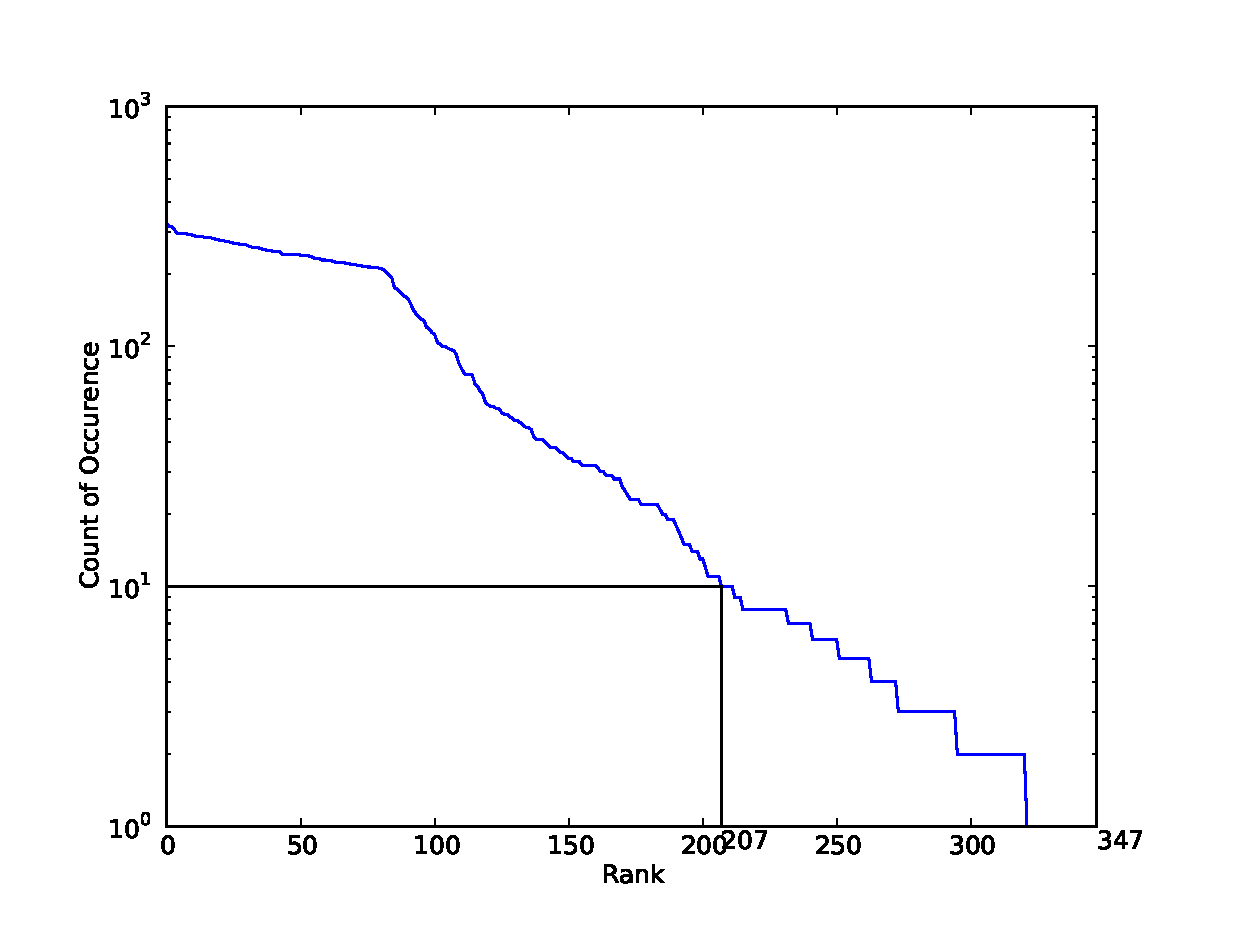
\epsfig{file=new_sample.eps, width=0.5\textwidth}
    \caption{The sample size of each combination (previous action, corresponding axis), 
    sorted from the most popular to least popular.  Mesh: Thai}
    \label{f:user:newsample}
\end{figure}

In Step 2, we need to determine $Pr(A_n |_{\textrm{current state}, A_n != A_p, An != \textrm{reverse}(A_p)})$
for each possible $A_n$. In this step, we ignore the effect of previous action. 
We think that $P_{continue}$ is high mainly because users tend to press the same key multiple times. 
It affects the $P_{change}$, but its effect on which action to be chosen as ``change'' is little.
%When a user has decided to go along another axis, we think the previous action has little effect on the choice of
%next action. 
Hence, we assume that $Pr(A_n |_{\textrm{current state}, A_n != A_p, An != \textrm{reverse}(A_p)})$
only depends on $(x, y, z, \theta_x, \theta_y, \theta_z)$. Here, all coordinates, except the corresponding coordinate
(it will not be changed since ``repeat'' and ``reverse'' are already excluded from the choices),
are important to decide the next action. 
We cannot directly derive the probability from the traces we collected because the sample size is not large enough.
%to derive the probabilities from the trace.
Instead, we propose a heuristic based on the assumption
\[
    Pr(x, y, z, \theta_x, \theta_y, \theta_z) = Pr(x)Pr(y)Pr(z)Pr(\theta_x)Pr(\theta_y)Pr(\theta_z)
\]
In other words, we assume that the probability for a viewpoint to have a specific coordinate is independent of its 
other coordinates. This is an assumption to simplify our model, and will introduce some difference between
synthetic traces and real traces. In the validation part, however, we show that the difference is not 
significant.

At a specific viewpoint $Vp$: $(x, y, z, \theta_x, \theta_y, \theta_z)$, if we change the value of $x$, 
then we stay in the 5-dimension space
\[
    (Y=y, Z=z, AX=\theta_x, AY=\theta_y, AZ=\theta_z).
\]
The probability of the viewpoint staying in this space is 
\begin{align*}
    &Pr(y, z, \theta_x, \theta_y, \theta_z)\\
    =&Pr(y)Pr(z)Pr(\theta_x)Pr(\theta_y)Pr(\theta_z)\\
    =&\frac{Pr(x)Pr(y)Pr(z)Pr(\theta_x)Pr(\theta_y)Pr(\theta_z)}{Pr(x)}\\
    =&\frac{Pr(x, y, z, \theta_x, \theta_y, \theta_z)}{Pr(x)}\\
    =&\frac{Pr(Vp)}{Pr(x)}.
\end{align*}
Similarly, we can know the probability of the viewpoint staying in other spaces. 

Hence, we set the probability of changing a value of a axis to be proportional to the probability of staying in the
corresponding space. For example, the probability of changing $x$ when the previous action is on $AY$
\begin{align*}
    =&\frac{\frac{Pr(vp)}{Pr(x)}}
            {\frac{Pr(vp)}{Pr(x)}
            +\frac{Pr(vp)}{Pr(y)}
            +\frac{Pr(vp}{Pr(z)}
            +\frac{Pr(vp)}{Pr(\theta_x)}
            +\frac{Pr(vp)}{Pr(\theta_z)}}\\
    =& \frac{\frac{1}{Pr(x)}}
            {\frac{1}{Pr(x)}
            +\frac{1}{Pr(y)}
            +\frac{1}{Pr(z)}
            +\frac{1}{Pr(\theta_x)}
            +\frac{1}{Pr(\theta_z)}
            }.
\end{align*}
Similarly, we can know the probability of changing other coordinates. Intuitively, we can think $Pr(x)$ as 
the popularity of current $x$ value. The above equation means that we tends to change the coordinate having low
popularity.

%We verify it with the traces we obtained and we can find that it is a reasonable simplification
%except for the first several viewpoints. 
%These first several viewpoints are the default viewpoint and its neighbors almost all users will pass, 
%so their probability is significantly higher. We ignore these points in this simplified method.
%Because we have enough samples for these viewpoints, we
%still use the standard method to derive the transition probability for these viewpoints. 

Next, for each axis we have two directions to move, and we need choose one.
We assume users tend to move to a direction with higher popularity, i.e. $Pr(vp)$. 
We define the popularity of a direction to be the sum of popularity of several consecutive positions in that direction
(we choose 3 positions in our implementation). 
Then, we assume the probability to go one direction is proportional to the popularity of that direction.
For example, if the axis to change is $X$ and its current value is $x$, 
the probability of moving right (considering three consecutive positions in that direction: $x+1$, $x+2$, $x+3$)
\begin{align*}
    =&\frac{\textrm{Popularity(right)}}
    {\textrm{Popularity(right)} + \textrm{Popularity(left)}} \\
   =&\frac{Pr(x+1)+Pr(x+2)+Pr(x+3)}
          {Pr(x+1)+Pr(x+2)+Pr(x+3)+Pr(x-1)+Pr(x-2)+Pr(x-3)}.
\end{align*}
Notice all these viewpoints have same $y$, $z$, $\theta_x$, $\theta_y$, and $\theta_z$, so they are not in
the equation. We consider several positions instead of one because users tend to repeat the same action several times,
so once a direction is chosen, the following several positions instead of one could be visited. 

In brief, we generate a synthetic trace as follows:
\begin{enumerate}
    \item Determine the session time according to the distribution of session time we derived from the real traces.
    \item For the default viewpoint, we derive the transition probability from the traces and decide the
        next action based on it.
    \item For other viewpoints, we choose ``repeat'', ``reverse'', or ``change'' 
        based on {previous action, corresponding coordinate}.
    \item If we choose ``change'', 
        we first determine the axis to change based on $Pr(x)$, $Pr(y)$, $Pr(z)$, 
        $Pr(\theta_x)$, $Pr(\theta_y)$, and $Pr(\theta_z)$. 
        Next, we choose the direction based on the popularity of three
        neighbors in both directions.
    \item We randomly select a think time from two different distributions 
        based whether the action is ``repeat'' or not (see Section \ref{ss:user:thinktime}).
        Then go back to step 3 unless the session time has expired.
\end{enumerate}

Based on our observations, the synthetic traces generated by our method satisfy some important requirements. 
When replaying the traces we generated, the mesh will not stay in abnormal state for long 
(abnormal positions include upside down, tilted, out of viewable area, etc.).
Since we determine $P_{repeat}$ and $P_{reverse}$ considering the corresponding coordinate,
the probability for the mesh to enter abnormal state is low, and it tends to go back to normal state
by ``reverse'' action. 
Moreover, whenever ``change'' is chosen, 
the mesh tends to go to a more normal state (a state having higher probability). 

\subsection{Comparison}
In this section, we compare the synthetic traces we generated with the real traces.
We generated 10000 synthetic traces following the simplified model we introduced in the last section.
Thai mesh is chosen as the mesh used in this validation because of its high complexity. Thai statue 
is the largest mesh and has many details, so more variety exist in users interactions. 

First, we compare the unconditional probability of each action in the traces. 
From Figure \ref{f:user:frequency_comp}, we can see that probability of each action in the traces we generated
fit well with that in the real traces. 
This result is impressing because we never consider unconditional probability in our model, but  
still the traces generated have similar unconditional probability for each action.
\begin{figure}[htdp!]
    \centering
    \epsfig{file=general_prob_comp.eps, width=0.5\textwidth}
    \caption{Comparison of occurrence frequency of each action.}
    \label{f:user:frequency_comp}
\end{figure}

Second, we compare the $P_{repeat}$, including unconditional $P_{repeat}$
and conditional $P_{repeat}$ under different previous action. We can see from Figure \ref{f:user:repeat_prob_comp},
the synthetic traces we generated has similar $P_{repeat}$ under all conditions.
\begin{figure}[htdp!]
    \centering
    \epsfig{file=repeat_prob_comp.eps, width=0.5\textwidth}
    \caption{Comparison of unconditional repeat probability and repeat probability under different previous actions.}
    \label{f:user:repeat_prob_comp}
\end{figure}

Third, we compare how the viewpoints distributed on each axis, 
i.e. the value of $Pr(x)$, $Pr(y)$, $Pr(z)$, $Pr(\theta_x)$, $Pr(\theta_y)$, and $Pr(\theta_z)$. 
Figure \ref{f:user:axis_distribution} shows that the synthetic traces we generated has similar distributions on all 
axises. Among the six axises, only the $Y$ axis has a slightly higher error. The synthetic traces tend to stay in the
center ($0$) more often. The correlation between these two set of values, however, is still close to $1$. 
Again, this result is interesting. Although we have considered these probabilities in selecting new action when
``change'' is selected, the majority of selections (recall that more than 80\% of actions are ``repeat'')
has nothing to do with these values. 
\begin{figure}[htdp!]
    \centering
    \begin{tabular}{cc}
    \epsfig{file=x.eps, width=0.45\textwidth}&
    \epsfig{file=y.eps, width=0.45\textwidth}\\
    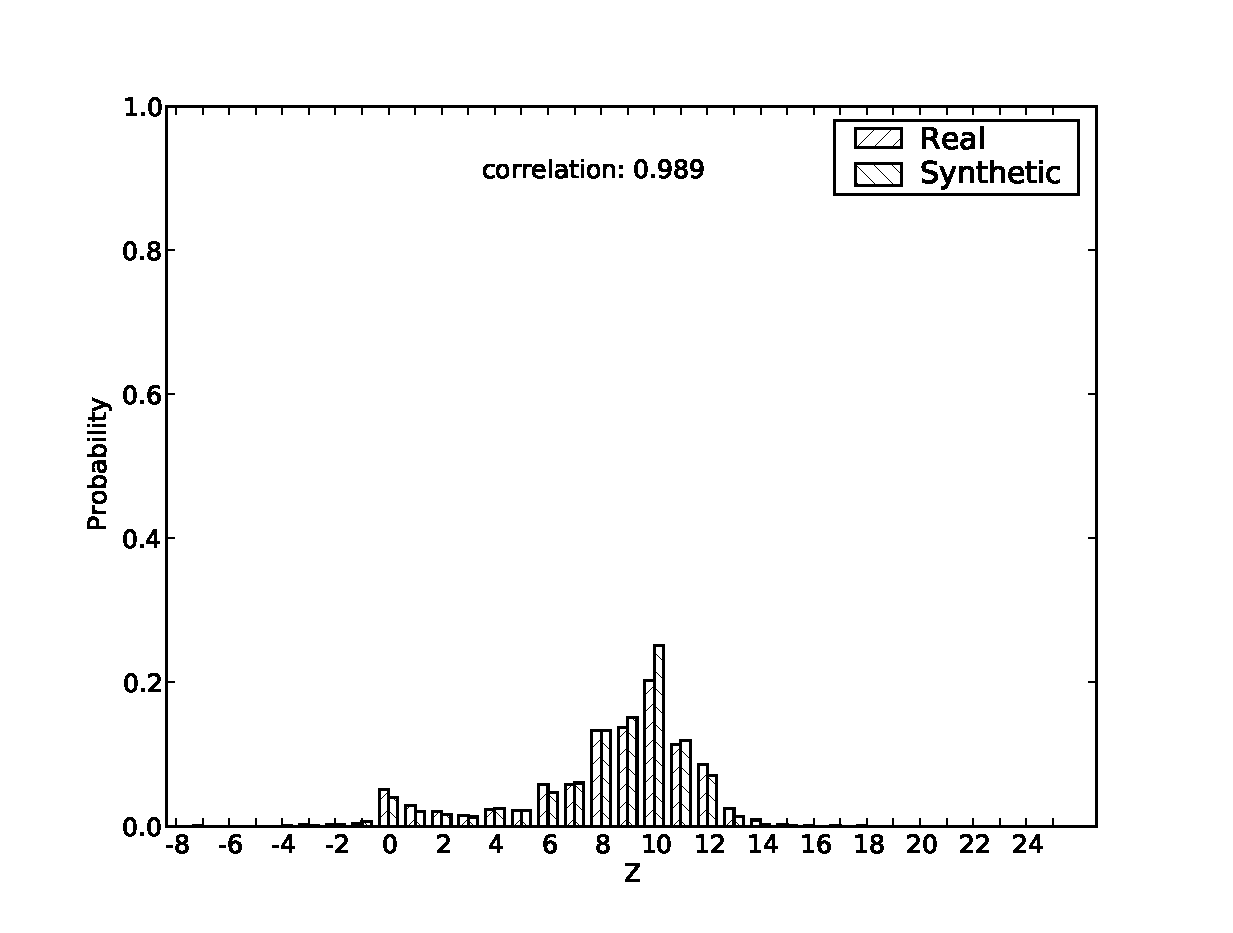
\epsfig{file=z.eps, width=0.45\textwidth}&
    \epsfig{file=ax.eps, width=0.45\textwidth}\\
    \epsfig{file=ay.eps, width=0.45\textwidth}&
    \epsfig{file=az.eps, width=0.45\textwidth}
    \end{tabular}
    \caption{Comparison of distribution of viewpoints on different axises.}
    \label{f:user:axis_distribution}
\end{figure}

The final comparison is on the transition probability on certain state, $Pr(A_n|_{(x, y, z, \theta_x, \theta_y, \theta_z, A_p)})$. 
If the Markov chain method is used, the synthetic traces should have the same transition probability with the real trace.
Due to the limited sample size, however, we have to use a simplified method. 
This comparison shows the difference introduced by this simplification. 
We only choose some states with enough number of samples to ensure the transition probabilities
are reliable. Some of the results are shown in Figure \ref{f:user:transition_comp}.
\begin{figure}
    \centering
    \begin{tabular}{cc}
        \epsfig{file=transition6.eps, width=0.45\textwidth}&
        \epsfig{file=transition8.eps, width=0.45\textwidth}\\
        \epsfig{file=transition10.eps, width=0.45\textwidth}&
        \epsfig{file=transition11.eps, width=0.45\textwidth}\\
        \epsfig{file=transition12.eps, width=0.45\textwidth}&
        \epsfig{file=transition16.eps, width=0.45\textwidth}\\
        \epsfig{file=transition17.eps, width=0.45\textwidth}&
        \epsfig{file=transition18.eps, width=0.45\textwidth}\\
    \end{tabular}
    \caption{Comparison of transition probabilities on certain states.}
    \label{f:user:transition_comp}
\end{figure}
In most of the cases, the synthetic traces have similar transition probability. The largest error happens
in the state (0, 0, 12, 0, 0, 0, ZOOM IN) 
when the sample size is small (22) and the distribution of next action is relatively even.
In this case, the transition probability derived from the real traces itself is not so reliable. 

In summary, due to the limited number of real traces, 
we cannot completely validate the synthetic traces we generated 
by checking the transition probability on each state.
According to the comparison we did, however,  
the synthetic traces we generated are similar to the real traces. 
Moreover, according to our observation, the traces we generated has much less
abnormal states (upside down, tilted, our of viewable area, etc.) than the random trace.
Therefore, we think it may be more realistic to use these synthetic traces rather than random traces to test the performance of
our mesh streaming system.

\section{Conclusion}
In this chapter we introduced how we generate synthetic traces based on real traces we collected.
These synthetic traces are similar with the real traces in the properties we compared.
Hence, we use them instead of random traces to measure the performance of the peer-to-peer 
mesh streaming system introduced in the next chapter.

%We conclude this chapter by showing some interesting preliminary findings we have.
With a preliminary analysis of the real traces we collected, we have obtained some
interesting findings.
First, in our usage scenario, user actions are predictable to certain extent. 
The prediction based on previous action is simple and effective. 
Therefore, it indicates pre-fetching is possible both in streaming and rendering within our scenario.
Second, our analysis reveals that in the traces we collected, 
locality exists in both data and viewpoint access. 
It may be possible to exploit this locality in 
designing progressive mesh streaming systems and rending systems.
%storing the most popular mesh data in caching proxies, the server overhead could be significantly reduced. 
%Third, we proposed a simple model to generate synthetic traces based on real traces we collected. 
%These synthetic traces are similar with the real traces in some properties we compared.
%Hence, they may be used in simulations to measure system performance without collecting
%a large number of traces.

While our original goal is to gather user traces to evaluate our system, 
our findings above, despite limited to a single usage scenario, 
points to a potentially important new research topic.  
Our study in this thesis establish the first step towards that direction.
